% IEEE Transactions on Cloud Computing — Revised Manuscript
% Transparent Multi-Cloud Migration Planning: A CSP–Expert–Pareto
%   Decision Pipeline
% Authors: Florin Olariu, Lenuța Alboaie, Cosmin Bonchiș
%
% REVISION NOTES (March 2026):
%   - Main comparison updated from 15-component/3-seed to 18-component/30-seed
%   - Paired t-tests + Cohen's d added (Section VI.C)
%   - Section VII: Netflix real-world case study added
%   - Sections VII–IX renumbered to VIII–X
%   - References ordered by first citation [1]–[39]

\documentclass[journal]{IEEEtran}

\usepackage{graphicx}
\usepackage{booktabs}
\usepackage{amsmath}
\usepackage{amssymb}
\usepackage{url}
\usepackage{xspace}
\usepackage{multirow}
\usepackage{array}
\usepackage{etoolbox}

% IEEEtran's \IEEEbiography environment inserts a "\vskip ... plus 1fil"
% before each biography block. Under the class's default \flushbottom
% (two-column) setting, that fil-stretch gets expanded to fill any leftover
% vertical space on a near-empty final column, producing very large gaps
% between the references and the first biography, and between consecutive
% biographies. We remove the stretch component so the gap stays a small,
% fixed size regardless of how much space remains on the page.
\makeatletter
\expandafter\patchcmd\csname\string\IEEEbiography\endcsname
  {\vskip \@IEEEBIOskipN plus 1fil minus 0\baselineskip}
  {\vskip \@IEEEBIOskipN minus 0\baselineskip}
  {}{\typeout{WARNING: IEEEbiography vskip patch did not apply}}
\makeatother

% --- Convenience macros --------------------------------------------------
\newcommand{\cmo}{CMO\xspace}
\newcommand{\cmothree}{CMOv3\xspace}
\newcommand{\cmofour}{CMOv4\xspace}
\newcommand{\ea}{EA\xspace}
% -------------------------------------------------------------------------

\begin{document}

\title{Transparent Multi-Cloud Migration Planning: A CSP--Expert--Pareto
  Decision Pipeline}

\author{Florin~Olariu, Lenu\c{t}a~Alboaie, and Cosmin~Bonchi\c{s}%
  \thanks{F.~Olariu and L.~Alboaie are with the Department of Computer Science,
  Alexandru Ioan Cuza University, Iasi, Romania
  (e-mail: florin.olariu@info.uaic.ro; lenuta.alboaie@info.uaic.ro).}%
  \thanks{C.~Bonchi\c{s} is with the Faculty of Computer Science, West
  University of Timisoara, Timisoara, Romania
  (e-mail: cosmin.bonchis@e-uvt.ro).}}

\maketitle

% =========================================================================
\begin{abstract}
Multi-cloud migration planning is a combinatorial decision problem in which
architects must satisfy hard constraints (budget, latency, provider
diversity) while justifying choices to technical and non-technical
stakeholders. Existing metaheuristic workflows can find good candidates, but
they often provide weak feasibility guarantees and limited explanation. We
present the Cloud Migration Optimizer (\cmo), a hybrid decision-support
framework that combines a constraint satisfaction layer for strict
feasibility filtering, an expert-rule layer for domain heuristics, Pareto
analysis for cost--latency trade-offs, and an interpretable multi-criteria
decision analysis (MCDA) layer over six quality criteria, together with an
explainability module producing constraint proofs, rule traces, and decision
paths.

We evaluate \cmo against several standard baselines, re-scoring every
method's output on the same six-dimensional MCDA objective for a fair
comparison. \cmo does not consistently dominate on this objective, or on raw
cost and latency, against a tuned genetic-algorithm baseline. \cmo's
advantage instead lies in properties a single scalar score cannot capture: a
deterministic, feasibility-guaranteed recommendation with a fully auditable
decision trail, neither of which the baselines provide. A real-world Netflix
streaming-architecture case study, built from public documentation and live
multi-cloud pricing, confirms this trade-off and shows \cmo consistently
satisfying provider-diversity constraints that the genetic-algorithm
baseline only meets intermittently. Overall, results indicate that a
constraint-centric hybrid pipeline trades a small, data-dependent gap in raw
optimisation quality for substantially improved determinism, feasibility
guarantees, and transparency, making it particularly suitable for regulated
and risk-sensitive migration contexts where a decision must be justified,
not just computed.
\end{abstract}

\begin{IEEEkeywords}
Cloud computing, multi-cloud migration, decision support systems, constraint
programming, multi-objective optimisation, Pareto frontier, explainable AI.
\end{IEEEkeywords}

% =========================================================================
\section{Introduction}
\label{sec:intro}

Cloud computing has evolved from single-provider infrastructure-as-a-service
deployments to complex ecosystems that span multiple providers, regions, and
managed services~\cite{armbrust_view,buyya_cloud,zhang_cloudstate}. Enterprise
architects now design application landscapes that might use an API gateway from
one provider, a managed database from another, and specialised analytics or AI
services from a third, sometimes within the same critical business flow. This
flexibility promises resilience and cost arbitrage. It also raises the difficulty
of making and justifying design decisions.

A multi-cloud migration project must satisfy hard constraints on total monthly
cost, end-to-end latency along key business transactions, and the number of
providers allowed by procurement or compliance policies. It must honour service
dependencies and compatibility constraints as well. At the same time, decision
makers care about softer objectives such as long-term reliability, security
posture, vendor lock-in risk, and scalability potential~\cite{zhang_cloudstate,
garg_framework}. The design space is combinatorial. Even an architecture with
fifteen logical components and a modest catalogue of service options per
component induces tens of millions of possible deployments.

Classical optimisation approaches for such problems include greedy heuristics,
genetic algorithms (GA), and evolutionary multi-objective algorithms like
NSGA-II and MOEA/D~\cite{deb_nsga2,zhang_moead,zeng_marketoriented}. They
are attractive because they can explore large spaces and provide approximate
Pareto fronts over competing objectives. Yet they have two important weaknesses
in the context of enterprise cloud migration. First, they are usually stochastic
and rely on penalty functions rather than exact constraint enforcement, so they
provide weak guarantees that all hard constraints are satisfied. Second, they
are largely opaque. They report final objective values but do not explain, in a
human-readable way, how and why a particular combination of services was chosen
over alternatives.

Decision-support practice in enterprises often moves in the opposite direction.
Architects use spreadsheets or static scoring matrices, manually weighting
attributes such as cost, performance, security, or compliance, in effect
implementing an ad-hoc multi-criteria decision analysis (MCDA) model without
formal normalisation~\cite{hwang_madm,saaty_ahp}. These artefacts are
interpretable. They do not scale to large configuration spaces, and they are
hard to validate or reproduce.

This paper argues that a hybrid approach can reconcile these tensions. The
central idea is to separate hard feasibility from soft preferences and to make
the decision pipeline itself an object of explanation. Cloud Migration Optimizer
(\cmo) is a system that embodies this idea. It uses a constraint satisfaction
problem (CSP) engine to eliminate infeasible configurations under budget,
latency, and provider diversity constraints. It then uses an expert rule system
and an optional normalised MCDA layer to evaluate feasible solutions along
economic and quality attributes. Finally, it applies Pareto analysis over cost
and latency to expose non-dominated trade-offs, and it presents the results
together with constraint proofs, rule traces, and decision paths that explain
why the recommended solutions are sound.

The implementation covers two related settings, denoted \cmothree and
\cmofour for brevity rather than as sequential software releases: \cmothree
exposes a fixed service catalogue and focuses on what might be called
incremental migration or re-hosting scenarios, while \cmofour introduces a
component-based architecture model that captures instance counts, technology
stacks, and dependency graphs. Both share the same core engines for
constraints, rules, Pareto metrics, and explainability, and differ only in
how latency is modelled (average-case versus critical-path); we treat them
as two configurations of one pipeline throughout, not as separate systems.

Relative to prior cloud-selection and multi-objective optimisation studies, the
novelty of \cmo is the tight integration of exact feasibility enforcement,
interpretable preference modelling, and traceable explanation in a single
auditable pipeline rather than in disconnected optimisation and reporting stages.

In summary, this article makes four main contributions. First, it defines a
concrete system and constraint model for multi-cloud migration planning that
can be solved with a constraint satisfaction engine using realistic cost and
latency models, including cross-region and cross-provider data-transfer prices
and critical-path latency. Second, it presents a hybrid CSP--Expert--Pareto
pipeline, implemented in an openly inspectable codebase, which separates hard
feasibility from soft preferences and combines rule-based scoring with
multi-objective Pareto analysis and an interpretable MCDA layer over six quality
metrics. Third, it introduces an explainability module that produces constraint
proofs, rule traces, decision paths, and visual artefacts such as cost and
latency Sankey diagrams and automatically generated PDF reports. Fourth, it
evaluates the approach empirically on synthetic yet realistic multi-cloud
architectures with up to eighteen components, comparing \cmo against five
baseline algorithms, including a tuned genetic algorithm, and it reports
detailed performance, frontier quality, and explanation metrics, together with a
statistical significance analysis over 30~independent runs and a validation and
sensitivity study. A real-world case study on the Netflix streaming architecture
further demonstrates generalisability.

% =========================================================================
\section{Background and Related Work}
\label{sec:related}

Cloud service selection and migration support has been widely studied, often
from the perspective of MCDA or metaheuristic optimisation. Many approaches
treat the problem as one of choosing among candidate services for a single
application or workload, typically aggregating criteria such as cost,
performance, availability, and security via weighted sums or outranking
methods~\cite{garg_framework,zhan_selection,han_multicriteria}. Others simulate
cloud environments and evaluate resource-provisioning algorithms at
scale~\cite{calheiros_cloudsim,buyya_intercloud}. A few works consider broker
architectures that mediate between consumers and providers in multi-cloud
settings~\cite{celesti_enhance,petcu_multicloud,menzel_cloudgenius}, although
they often focus on interface and orchestration concerns more than on deep
optimisation and decision explanation.

Multi-objective optimisation in cloud computing frequently relies on genetic
algorithms and their variants. Studies have applied NSGA-II to virtual machine
placement, energy-aware scheduling, web service composition, and workflow
optimisation~\cite{deb_nsga2,zeng_marketoriented,wu_market}. MOEA/D and other
decomposition-based algorithms have also been explored for resource allocation
problems~\cite{zhang_moead}. Such methods can approximate Pareto fronts across
conflicting goals. They remain black-box search processes in most deployments,
which makes them hard to justify to stakeholders beyond their numerical outputs.

MCDA methods such as the Analytic Hierarchy Process (AHP)~\cite{saaty_ahp},
TOPSIS~\cite{hwang_madm}, PROMETHEE~\cite{brans_promethee}, and
ELECTRE~\cite{roy_electre} have been applied to cloud service selection as well.
For example, Garg and Buyya describe a framework that ranks cloud services based
on quality-of-service (QoS) attributes using AHP and related
techniques~\cite{garg_framework}. Other studies propose MCDA-based cloud brokers
that allow users to specify weights and thresholds on non-functional
properties~\cite{zhan_selection,han_multicriteria}. These approaches tend to
operate over small, manually curated sets of alternatives. They handle weights
and normalisation explicitly, which helps interpretability, but they rarely
integrate with a combinatorial search layer that enumerates feasible
configurations.

Constraint programming has a long history in scheduling and resource
allocation~\cite{rossi_handbook,baptiste_csp}. It provides expressive modelling
of hard constraints and can integrate with optimisation criteria, using search
strategies to exclude infeasible or dominated regions of the space. Applied to
cloud computing, CSP and related exact methods have been used for SLA-aware
resource allocation, workflow placement, and data centre
management~\cite{sharma_sla,fersman_csp}. Many such systems target
single-provider or homogeneous environments. They do not always combine CSP with
explainable rule systems or MCDA-like preference layers.

Explainable artificial intelligence (XAI) has focused predominantly on
supervised learning models~\cite{ribeiro_lime,guidotti_survey,doshi_rigorous}.
There is, however, a growing interest in explainability for optimisation and
decision-support systems, particularly in operations research and multi-criteria
analysis~\cite{miettinen_multiobjective,schoen_explainable,hauser_explanatory}.
Work in this area often proposes interactive visualisations of Pareto fronts,
sensitivity analysis for weights, or ex post explanations of chosen solutions,
sometimes using rule-based or example-based narratives.

Additional strands of work address QoS prediction for cloud
services~\cite{han_qos}, measurement-based comparisons of
providers~\cite{leitner_service,li_cloudcmp}, design patterns and metrics for service-based
systems~\cite{morasca_measuring}, and broker frameworks such as InterCloud that
manage utility-oriented federations of cloud
environments~\cite{buyya_intercloud}. These contributions highlight the need for
systematic evaluation and informed decision making in cloud contexts. They also
show how difficult it is to reconcile technical optimisation with human
understanding.

The Cloud Migration Optimizer builds on these strands but integrates them in a
specific way. It takes the CSP paradigm seriously for constraint enforcement,
uses an expert rule engine to represent soft best-practice knowledge, leverages
Pareto analysis for multi-objective cost--latency trade-offs, and exposes an
MCDA-style normalised scoring model over six metrics. At the same time, it
emphasises explainability by design, providing machine-generated proofs of
constraint satisfaction, explicit rule firing logs, and visual flow diagrams
that can be consumed by both technical and non-technical stakeholders. This
combination is less common in existing cloud service selection tools, which tend
to prioritise either search effectiveness, user-friendly scoring, or interactive
visualisation in isolation.

% =========================================================================
\section{System Model and Problem Statement}
\label{sec:model}

The Cloud Migration Optimizer considers an enterprise application decomposed
into logical components, together with a set of cloud service options for each
component, and a collection of global constraints and preferences. The system
must select one concrete service implementation for each component, such that
all constraints are satisfied and such that the resulting architecture lies on
or near a cost--latency Pareto frontier and aligns with user preferences over
reliability, security, lock-in risk, and scalability.

An architecture is represented as a set of components
\begin{equation}
  C = \{c_1, c_2, \ldots, c_n\}.  \label{eq:components}
\end{equation}
Each component $c_i$ has an associated type, for example API gateway,
application server, relational database, NoSQL store, cache, message queue,
event streaming engine, storage bucket, monitoring service, backup, CDN,
identity provider, encryption service, container orchestration, or serverless
runtime. Each component also has an instance count and a record of its
technology stack, such as programming language, framework, or storage engine.
Components are connected by directed dependency edges that represent calls or
data flows, such as a user-facing front-end depending on an application server,
or a cache depending on a database.

For each component $c_i$ there is a set of concrete service options
\begin{equation}
  S_i = \{s_{i1}, s_{i2}, \ldots, s_{ik_i}\}  \label{eq:options}
\end{equation}
drawn from AWS, Azure, and Google Cloud catalogues. A deployment configuration
is a mapping
\begin{equation}
  f : C \to S, \qquad f(c_i) \in S_i,  \label{eq:config}
\end{equation}
which chooses one service for each component. Derived from $f$ is a provider
set $P(f)$ that records which cloud providers appear in the configuration.
Derived as well is a component--service configuration that can be translated
into infrastructure-as-code templates, such as Terraform modules, for
deployment.

A configuration must satisfy several hard constraints. First, there is a
monthly budget limit $B_{\max}$ on total cost. The cost function
$\mathrm{cost}(f)$ aggregates per-service prices, which include compute
instance charges, managed database rates, storage costs, per-request charges
for API gateways, and data-transfer charges across availability zones, regions,
and providers. Workload profiles specify expected request volumes and
data-transfer amounts, and cost contributions are computed using live or
documented pricing data when available. Second, there is an end-to-end latency
limit $L_{\max}$ for key request flows. The latency function $\mathrm{lat}(f)$
can be instantiated as a weighted average across component latencies or, more
realistically, as the critical-path latency of a dependency graph, where node
processing times and edge network latencies depend on chosen regions and
providers. Third, there is a provider diversity constraint that restricts the
number of distinct providers in $P(f)$ to at most $P_{\max}$, thereby enforcing
organisational policies about multi-cloud exposure. Service-dependency and
compatibility constraints are also enforced.

Formally, the feasible set is
\begin{equation}
  \mathcal{F} = \left\{ f \;\middle|\;
  \begin{array}{l}
    \mathrm{cost}(f) \le B_{\max}, \\
    \mathrm{lat}(f) \le L_{\max}, \\
    |P(f)| \le P_{\max}, \\
    \text{all service dependencies satisfied}
  \end{array}
  \right\}.  \label{eq:feasible}
\end{equation}
Within $\mathcal{F}$ the primary optimisation objectives are cost and latency.
For each feasible configuration, the system also estimates a reliability score
$r(f) \in [0,1]$ based on provider SLAs and service type reliability
multipliers, a security score $s(f) \in [0,1]$ reflecting encryption, identity
management, and compliance features, a vendor lock-in risk score
$v(f) \in [0,1]$ where higher values indicate greater risk, and a scalability
score $q(f) \in [0,1]$ based on the presence of serverless, container, and
load balancing services. These metrics are not part of the primary CSP
feasibility region, but they guide expert rules and MCDA ranking.

The goal of \cmo is therefore twofold. The system must find a diverse set of
feasible configurations that approximate the cost--latency Pareto frontier for
the given constraints and architecture. It must also explain, with structured
evidence, why particular configurations, and especially the top-ranked
recommendations, constitute good trade-offs according to user preferences and
best practices.

% =========================================================================
\section{Hybrid CSP--Expert--Pareto Optimisation Pipeline}
\label{sec:pipeline}

The optimisation pipeline in \cmo consists of three main stages. The first
stage is a constraint satisfaction engine that generates feasible solutions
under the given cost, latency, and provider constraints. The second stage is an
expert rule system together with an optional MCDA model that evaluates the
quality of each feasible solution beyond mere feasibility. The third stage is a
Pareto frontier module that extracts non-dominated solutions in cost--latency
space and computes metrics for analysing frontier quality.

\subsection{Constraint Satisfaction Engine}
\label{sec:csp}

The CSP engine operates over an implicit search tree where each level
corresponds to choosing a concrete service for one component. It uses a
combination of exhaustive enumeration, heuristic candidate construction, and
random sampling, depending on the architecture size and time budget. For very
small architectures, such as those with five components and a limited set of
options, the engine can enumerate the entire Cartesian product of service
options and filter each configuration for feasibility. For larger architectures
with ten or fifteen components and richer catalogues, exhaustive enumeration is
infeasible. In those cases, the engine builds candidate configurations using
heuristics that favour low-cost or low-latency options subject to constraints,
and it supplements this strategic sampling with bounded random sampling to
improve diversity.

For each partial or complete configuration, the engine computes a cost and a
latency estimate using pricing and latency models. Pricing is derived from a
service data cache that fetches live Azure retail prices and uses documented AWS
and GCP rates as fallbacks~\cite{azure_prices,aws_pricing,gcp_pricing}. When
live data retrieval fails or is slow, the system can revert to cached or
fallback prices, ensuring that optimisation remains responsive. Latency is
computed either as an average across component latencies or, in the \cmofour
extended model, as the critical path of a directed graph whose nodes represent
services and whose edges represent call or data dependencies. Each edge latency
is the sum of a network component, which depends on the source and target
regions, and a service processing latency associated with the target.

Configurations that violate any hard constraint are immediately discarded. This
includes those whose minimum possible cost, estimated by selecting the cheapest
option per component, already exceeds the budget, which can be detected early.
The CSP engine also enforces provider count and dependency constraints. Only
those configurations that pass all checks are wrapped into \texttt{Solution}
objects with attributes for configuration mapping, total cost, latency, provider
count, and provider distribution. These objects populate the feasible
set~$\mathcal{F}$.

To prevent runaway computations, the CSP engine can be run under a global
timeout mechanism. \cmofour uses a thread-based timer that flips a shared flag
when the time budget is exceeded, and the search adheres to this flag at safe
points. In addition, the engine logs search statistics such as the total number
of theoretical combinations, the number of feasible solutions found, and the
proportion of configurations eliminated by constraints.

We state the resulting guarantee precisely, since it is easy to overstate.
\cmo guarantees that every solution it returns is feasible with respect to
all stated hard constraints (budget, latency, provider count, and
dependencies): a returned solution is never subsequently found to violate a
constraint, by construction. For architectures small enough for exhaustive
enumeration (five components in this study), \cmo additionally guarantees
completeness: the returned feasible set and Pareto frontier are exactly
the true feasible set and true Pareto frontier. For larger architectures
(ten components and above, including all scenarios reported in
Sections~\ref{sec:multirun} and~\ref{sec:netflix}), the engine relies on
heuristic construction and bounded sampling rather than exhaustive search, so
\emph{feasibility of returned solutions is guaranteed but completeness of the
feasible set or Pareto frontier is not}: there may exist feasible or
non-dominated configurations that the engine does not enumerate.

\subsection{Expert Rule System}
\label{sec:expert}

Once feasible solutions have been identified, \cmo applies an expert rule
system implemented using the \texttt{experta} framework. Each solution is
encoded as a fact with attributes including cost, latency, provider count, main
provider, and a preferences structure capturing whether the user prioritises
cost savings, performance, or a specific provider.

The rule base consists of several categories. Cost-focused rules define
thresholds for high, moderate, and low costs, relative either to absolute
values or to the budget. Solutions whose cost exceeds a high threshold incur
penalties, while those below a low threshold receive rewards. Latency-focused
rules reward solutions whose latency is well below the limit and penalise those
that approach or exceed it. Strategic rules examine provider count and
distribution. They may reward single-provider deployments for operational
simplicity or dual-provider deployments for a balance between diversification
and complexity, while penalising configurations that use three providers without
corresponding latency benefits. Some strategic rules also look for balanced
provider distributions that avoid having more than a fixed fraction of
components on any single provider, thereby mitigating vendor lock-in risk.

Preference rules tailor scoring to user priorities. If the user indicates a
preferred provider, solutions where the majority of components run on that
provider receive additional points. If the user prioritises cost, then low-cost
solutions receive amplified rewards, whereas performance-prioritising users
receive larger bonuses for low-latency solutions.

In addition to these general rules, \cmofour introduces component-specific
rules for patterns such as cache usage, content delivery networks, message
queues, backups, monitoring, containers, and serverless platforms. For example,
a rule may reward the presence of a cache when overall latency is below a
certain threshold, indicating that caching is effectively improving performance,
or it may reward message queues that enable asynchronous processing in
cost-effective configurations.

The rule engine initialises each solution with a baseline score, typically 100,
and then applies rules in a forward-chaining manner. Each triggered rule adds
or subtracts a certain number of points, scaled by a category weight. At the
end of inference, each solution has both a raw score and a capped score, the
latter kept in a suitable range for display. The engine also records a log of
all fired rules, including their names, categories, weights, score
contributions, and evidence details such as observed cost and latency versus
thresholds.

This rule trace is central to explainability. It provides a structured account
of which qualitative considerations led to the final score and thus to the
ranking of solutions. Because the rules are parameterised by thresholds and
weights that can be adjusted, the system also supports tuning for different
organisational contexts.

\subsection{Normalised MCDA Layer}
\label{sec:mcda}

While rule-based scores capture relative quality in an expert-system fashion,
some scenarios benefit from more principled multi-criteria aggregation. The
\cmo codebase therefore includes a normalised MCDA module that acts on top of
feasible solutions and their extended metrics. For each solution, the system
computes six raw metrics: total monthly cost, end-to-end latency, security
score, vendor lock-in score, scalability score, and reliability score. These
are then normalised across the set of feasible solutions using min--max scaling.

Normalisation proceeds as follows. For each metric, the minimum and maximum
values across all feasible solutions are identified. The normalised value is
computed as
\begin{equation}
  \hat{x} = \frac{x - x_{\min}}{x_{\max} - x_{\min}}.  \label{eq:minmax}
\end{equation}
If the range $x_{\max} - x_{\min}$ is zero, indicating that all solutions have
the same value for that metric, the normalised value is set to $\hat{x} = 0.5$
to reflect a neutral middle position. The system clamps all normalised values
into the $[0,1]$ interval and handles numerical edge cases gracefully.

Not all metrics are interpreted in the same direction. For cost, latency, and
vendor risk, lower is better, so the MCDA model uses $1 - \hat{c}$,
$1 - \hat{\ell}$, and $1 - \hat{v}$, where hats denote normalised values. For
reliability, security, and scalability, higher is better, so the model uses the
normalised values $\hat{r}$, $\hat{s}$, and $\hat{q}$ directly.
User-specified weights $w_c, w_\ell, w_r, w_s, w_v, w_q$ that sum to unity
control the relative importance of these metrics. The final MCDA score is
\begin{align}
  \mathrm{score}_{\mathrm{MCDA}} &= w_c(1 - \hat{c}) + w_\ell(1 - \hat{\ell})
    \nonumber \\
  &\quad + w_r\hat{r} + w_s\hat{s} \label{eq:mcda} \\
  &\quad + w_v(1 - \hat{v}) + w_q\hat{q}. \nonumber
\end{align}
The implementation supports default weights of 30\% for cost, 20\% for
latency, 20\% for reliability, 15\% for security, 10\% for vendor risk, and
5\% for scalability, which reflect a balanced enterprise setting where economic
and performance considerations dominate but other aspects still matter. This
default was set from practitioner priority ordering rather than fitted to any
particular dataset: cost and latency are the two criteria migration
stakeholders consistently name first in scoping conversations and are also the
two criteria every baseline in this study can be meaningfully compared on,
which motivates their combined 50\% weight; reliability and security are
weighted next (20\% and 15\%) because they are typically treated as
non-negotiable floors rather than optimisation targets in enterprise
procurement; vendor lock-in risk (10\%) and scalability (5\%) receive the
smallest weights because they matter most over a longer time horizon than the
other four criteria, which this single-snapshot evaluation cannot capture.
Alternative profiles, such as cost-focused, performance-critical,
security-first, or vendor-risk-averse configurations, can be represented by
adjusting these weights, and Section~\ref{sec:mcdasensitivity} reports how
sensitive the ranking of methods is to exactly this kind of adjustment.

An important feature of this MCDA layer is that it exposes the normalisation
ranges and weights in the user interface and in exported data. This transparency
helps stakeholders understand not only the final scores but also the underlying
trade-offs between metrics. The MCDA model does not replace the Pareto frontier
computation. Instead, it provides a scalar summary that can be useful for quick
ranking or when a single recommended solution is required.

\subsection{Weight Sensitivity}
\label{sec:mcdasensitivity}

Because the MCDA ranking in Table~\ref{tab:mcda-baselines} depends on the
chosen weights, we tested how robust that ranking is to a stakeholder
adopting a different priority ordering. We re-scored the same six methods'
returned solutions on the same pool, under five named weight profiles: the
balanced default above, plus cost-focused (55\% cost), performance-critical
(55\% latency), security-first (45\% security), and vendor-risk-averse (50\%
vendor risk), each redistributing the remaining weight across the other
criteria. Table~\ref{tab:mcda-sensitivity} reports the top-ranked method under
each profile.

\begin{table}[t]
\centering
\caption{Top-Ranked Method by MCDA Weight Profile (18-component scenario;
pricing snapshot 26~Sep~2026)}
\label{tab:mcda-sensitivity}
\begin{tabular}{@{}lll@{}}
\toprule
Weight Profile          & Top Method    & Score \\
\midrule
Balanced (default)      & GA            & 0.7645 \\
Cost-focused            & GA            & 0.8296 \\
Performance-critical    & Greedy-Latency & 0.6745 \\
Security-first          & GA            & 0.6572 \\
Vendor-risk-averse      & Greedy-Cost   & 0.8261 \\
\bottomrule
\end{tabular}
\end{table}

\cmofour does not top the ranking under any of the five profiles tested,
including vendor-risk-averse, where it finishes a close second (0.8200 vs.\
0.8261) to Greedy-Cost. Inspecting the six raw per-criterion scores explains
why: on this eighteen-component architecture, all six methods' returned
solutions attain identical reliability (1.00), security (1.00), and
scalability (0.658) scores, because every feasible solution in this
constraint set already satisfies these three criteria at their ceiling value.
The MCDA score therefore has effective discriminating power on only three of
its six dimensions here (cost, latency, and vendor lock-in risk), and
\cmofour's advantage on the third of these (vendor risk 0.333 vs.\ GA's 0.5)
is consistently too small to offset its higher cost, even when vendor risk is
given 50\% of the total weight. We report this as an honest limitation of
scalar MCDA comparison rather than obscuring it: it further supports the
position taken in Section~\ref{sec:multirun} and
Section~\ref{sec:discussion} that \cmo's value in this evaluation lies in
feasibility guarantees, determinism, and auditability rather than in
topping any particular weighting of a six-dimensional score, a distinction
that only becomes visible once reliability, security, and scalability stop
discriminating between candidate solutions, as they do in this architecture.
A more heterogeneous catalogue of service options, where reliability and
security genuinely trade off against cost rather than being uniformly
available at the ceiling level for every provider combination, would be a
natural next step for making the reliability and security weights consequential
in practice; we note this as future work.

\subsection{Pareto Frontier and Metrics}
\label{sec:pareto}

Independently of rule-based or MCDA scores, \cmo computes the cost--latency
Pareto frontier over feasible solutions. A solution $f_a$ is said to dominate
another solution $f_b$ if it is no worse in both cost and latency and strictly
better in at least one. The frontier consists of all feasible solutions that are
not dominated by any other solution. Computing this frontier involves checking
each candidate against all others, though in practice the number of feasible
solutions is modest enough that a straightforward non-dominated filtering
algorithm suffices.

The Pareto module also calculates several indicators that characterise the
quality and diversity of the frontier. The hypervolume indicator measures the
volume of objective space dominated by the frontier with respect to a reference
point, typically chosen slightly beyond the worst observed cost and latency. In
the two-objective case, this reduces to an area computation obtained by sorting
frontier solutions by cost and summing rectangles. The spacing metric computes
the standard deviation of distances between consecutive frontier points when
sorted by cost, providing a sense of how evenly they are distributed. The
module also identifies extreme solutions: the minimum-cost solution, the
minimum-latency solution, and a balanced solution that is closest to the ideal
point of minimum cost and minimum latency in normalised space.

These metrics are used primarily in the experimental analysis. They help compare
\cmo's frontiers with those produced by evolutionary baselines and assess
whether the frontier offers a rich set of trade-offs or collapses into a single
dominant configuration.

% =========================================================================
\section{Explainability and Reporting}
\label{sec:explain}

Explainability in \cmo is designed as a parallel set of artefacts that mirror
the main stages of the pipeline. Whenever the system runs an optimisation, it
can generate constraint proofs, rule traces, decision paths, and visual
representations that together form a multi-layered explanation.

Constraint proofs document how each hard constraint was evaluated for a given
solution. They record the required value, the actual value, a Boolean
satisfaction flag, and a margin indicating how far within or beyond the limit
the solution lies. For the budget constraint, this means showing the total
monthly cost, the budget limit, and the absolute difference. For the latency
constraint, it means showing the computed latency, the threshold, and the
margin. Provider diversity checks record the number of providers used and
compare this with the maximum allowed, while component coverage checks ensure
that all required components have assigned services. These proofs can be seen as
structured certificates that a solution is mathematically feasible.

To make this concrete rather than abstract, we quote below the constraint
proof that \cmo's explainability module emits, verbatim and unedited, for a
feasible solution on the eighteen-component enterprise architecture under the
same constraints used throughout Section~\ref{sec:experiments} (budget
\$5{,}000/month, latency limit 150\,ms, maximum 3 providers). This particular
solution (\$808.61/month, 20.50\,ms, 3 providers: 10 AWS, 7 GCP, 1 Azure) was
generated fresh for this illustration rather than copied from
Table~\ref{tab:mcda-baselines}; because pricing is fetched live at query
time, its specific cost differs from the pricing-snapshot figures reported
elsewhere in this paper, but the proof's structure and wording are exactly
what the module emits for every solution discussed in this paper.

\begin{itemize}
  \item \textit{Maximum Budget}: Solution cost \$808.61 is within budget limit of \$5000 by \$4191.39.
  \item \textit{Maximum Latency}: Solution latency 20.50ms is within limit of 150ms by 129.50ms.
  \item \textit{Maximum Providers}: Solution uses 3 providers (GCP: 7, AWS: 10, Azure: 1), within limit of 3.
  \item \textit{Component Coverage}: All required components assigned.
\end{itemize}

Each line above is generated automatically from the solution's own
attributes by the function reproduced in Section~\ref{sec:csp}, not
hand-written per case, so the same certificate format accompanies every
recommendation \cmo returns throughout this paper. We present this as a
concrete illustration of the artefact's content and format, not as empirical
evidence that it improves a practitioner's decision; we return to that
distinction, and to what would be needed to test it, in
Section~\ref{sec:threats}.

Rule traces are built directly from the expert rule engine's evaluation log.
For each fired rule, the trace contains the rule name and category, the weight,
the score contribution, and a short textual reasoning string, often combined
with evidence in the form of observed values and thresholds. For example, a
low-cost reward rule might record that the solution cost is under 40\% of
budget and thus deserves a positive adjustment, while a high latency penalty
might note that the latency exceeds 90\% of the limit. Traces can be inspected
in the user interface or exported as part of an API response.

Decision paths summarise the entire optimisation process in a sequence of
human-readable steps. A typical decision path begins with input validation,
which confirms that the specified budget, latency, and provider limits are
within plausible ranges. It then reports the size of the search space in terms
of the number of theoretical configurations, based on the number of components
and options per component. Next, it provides CSP filtering statistics, including
the number of feasible solutions and the percentage of configurations eliminated
by constraints. The path then describes Pareto frontier computation, stating how
many non-dominated solutions were found and what proportion they represent among
feasible solutions. It continues with expert ranking, summarising rule
categories and high-level patterns. Finally, it reports the selected
recommendation, including its cost, latency, and score, and emphasises that all
constraints are satisfied.

Beyond textual artefacts, \cmo generates visual explanations. Cost Sankey
diagrams~\cite{riehmann_sankey} illustrate how cost flows from providers through
component categories to total cost. Providers are represented as upstream nodes,
component categories such as compute, data, network, security, and operations
occupy intermediate nodes, and flow thickness encodes cost contributions. This
helps users see which providers and categories are the main cost drivers.
Latency-based Sankey diagrams take a similar structure but encode latency
instead of cost, focusing on individual components rather than categories.

Fig.~\ref{fig:sankey_cost} shows the cost Sankey diagram for the balanced
\cmothree/\cmofour solution. The flows from AWS and GCP to compute, data,
network, security, and operations categories make immediately clear which
providers and component classes dominate the monthly cost.

For critical-path latency analysis, the system can render graphs of service
dependencies, highlighting the longest latency path and annotating each hop
with service and network latency contributions. These diagrams convey why two
configurations with similar average latencies might differ in tail latency
behaviours, which is often important for user experience.

All of these artefacts are consumed by an academic-style report generator
implemented using the ReportLab library. The generator builds a PDF document
that includes a title page, executive summary, technical architecture
description, financial analysis, selection rationale, explainability section,
and recommendations. It integrates constraint proofs, rule traces, decision
paths, and visualisations, providing a cohesive narrative suitable for
reviewers, auditors, or technical steering committees.

\begin{figure}[t]
  \centering
  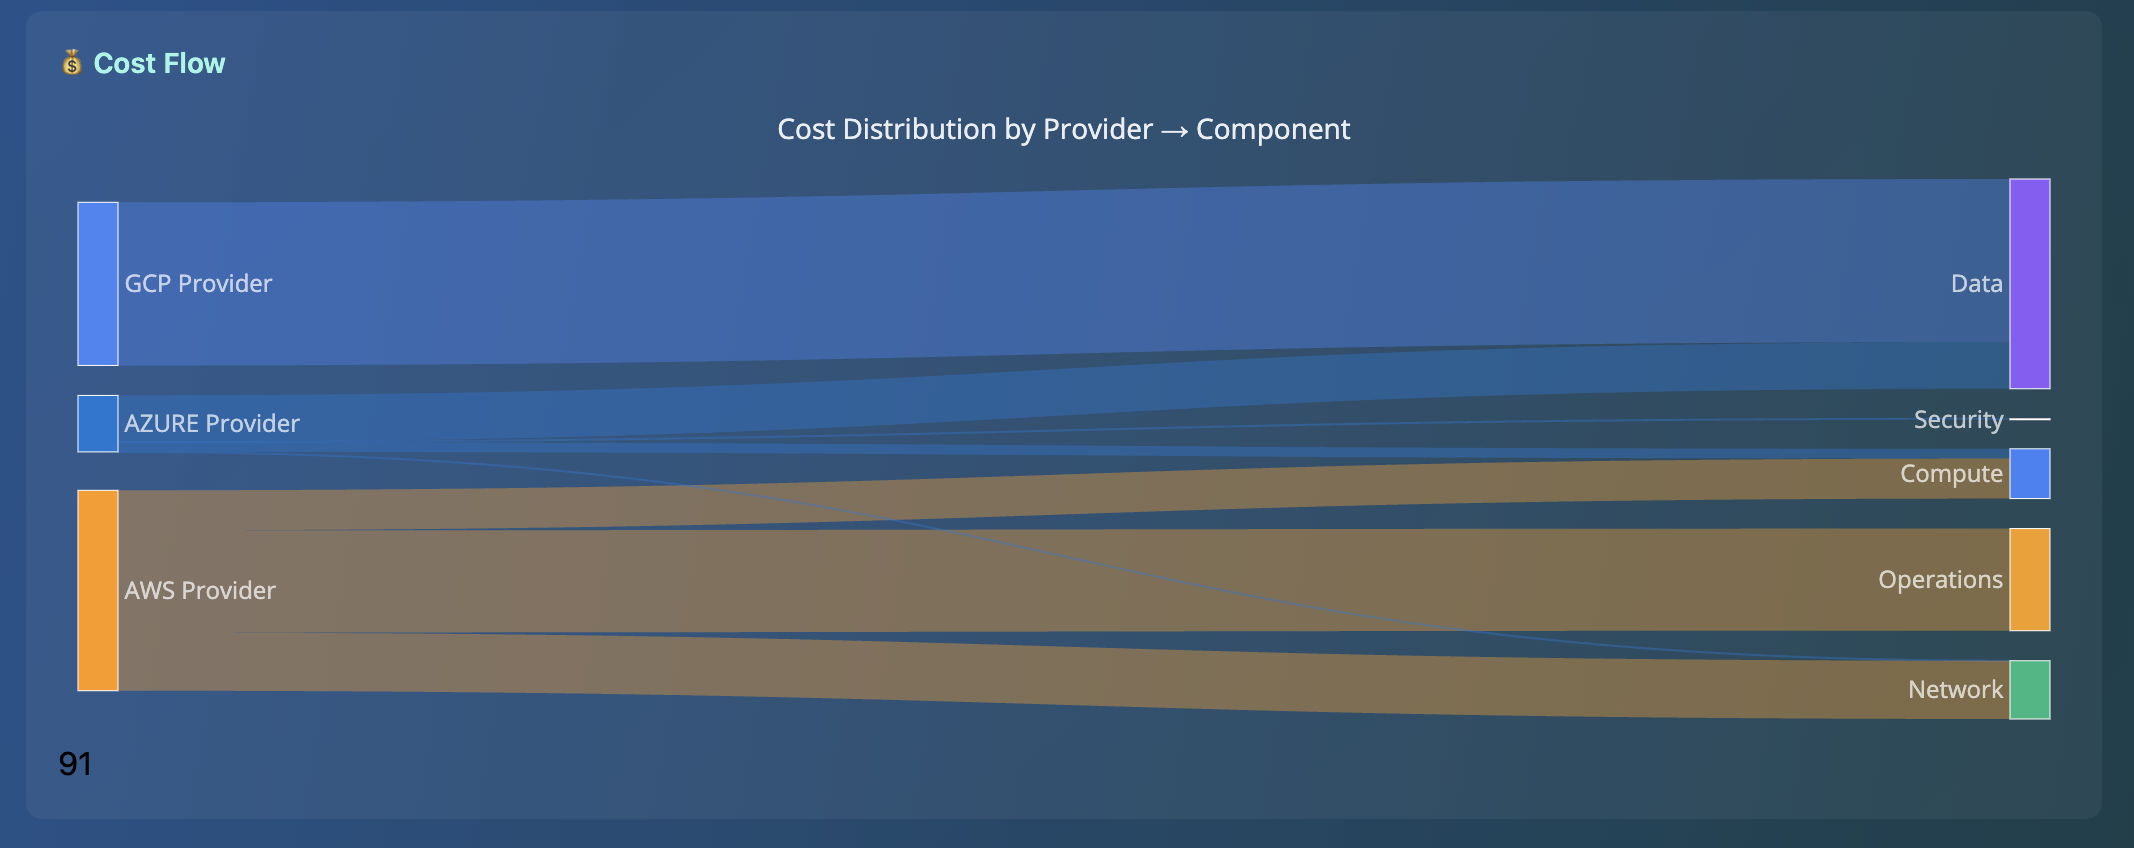
\includegraphics[width=0.95\columnwidth]{figs/sankey_cost.png}
  \caption{Cost flow Sankey diagram for the balanced \cmothree solution
  (\$974.68/month, two providers). Flow width encodes monthly cost contributions
  from providers to component categories.}
  \label{fig:sankey_cost}
\end{figure}

\begin{figure}[t]
  \centering
  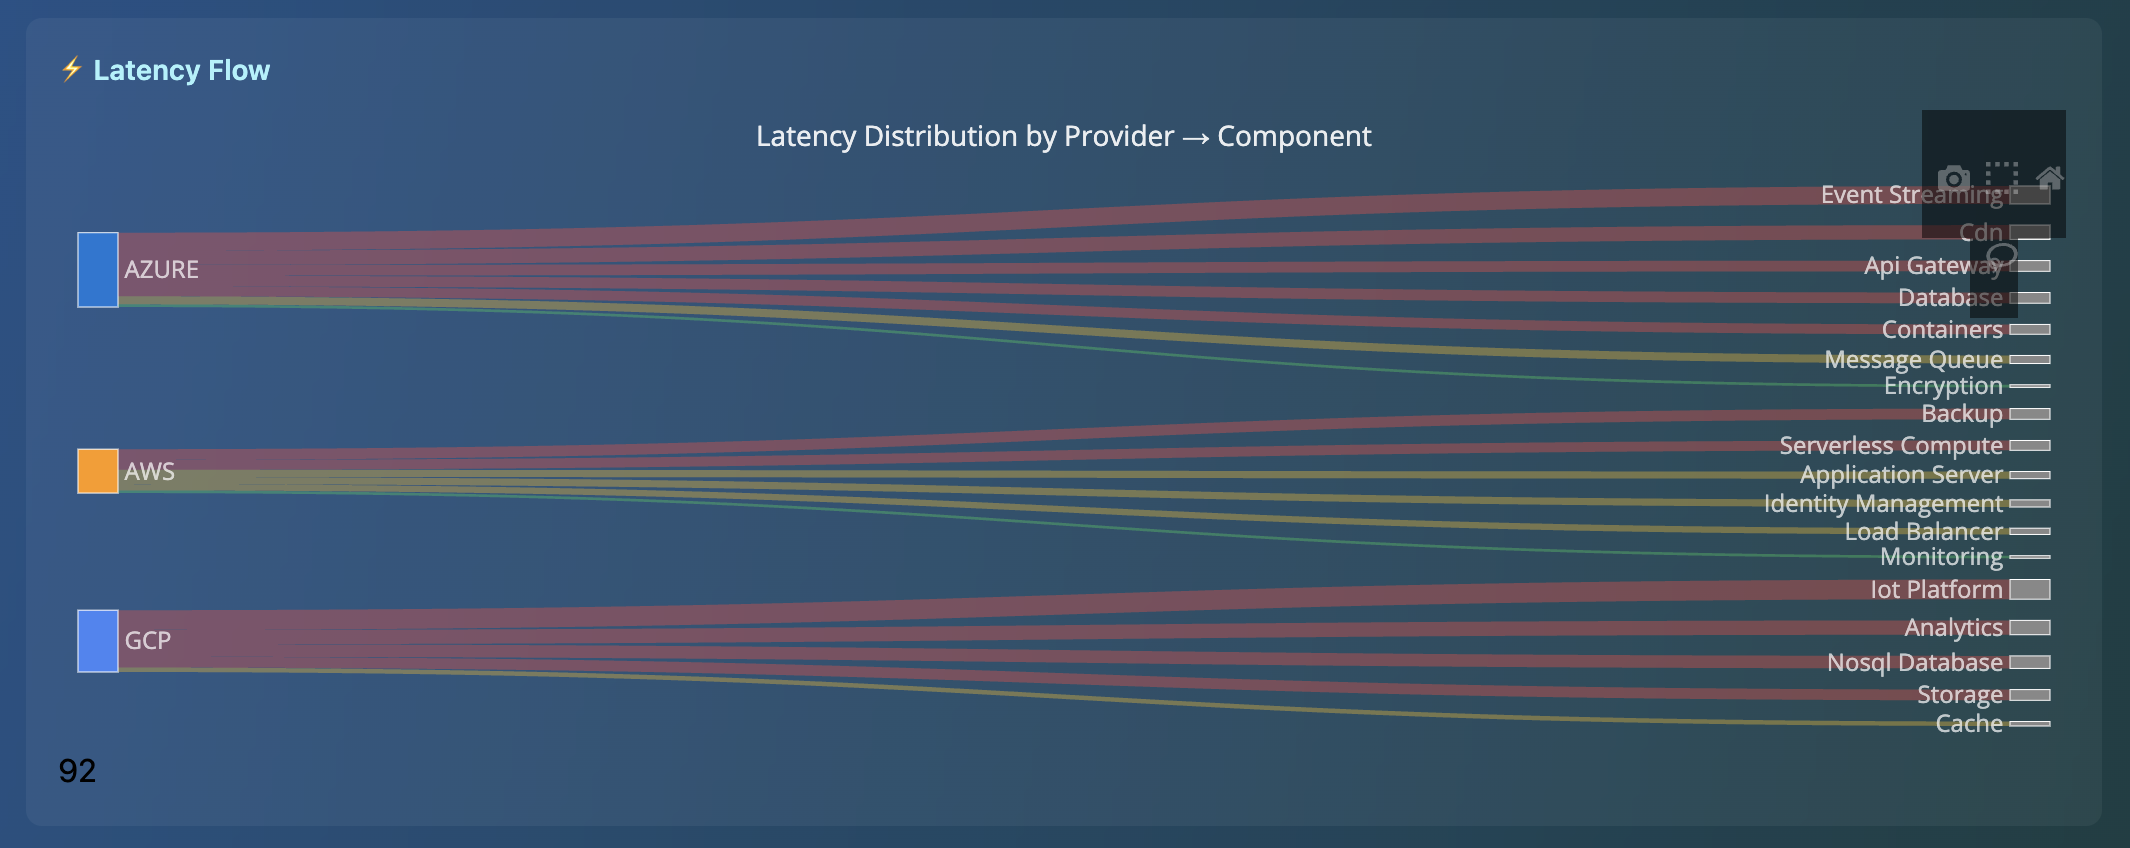
\includegraphics[width=0.95\columnwidth]{figs/sankey_latency.png}
  \caption{Latency flow Sankey diagram for the balanced \cmothree/\cmofour
  solution.}
  \label{fig:sankey_latency}
\end{figure}

% =========================================================================
\section{Experimental Evaluation}
\label{sec:experiments}

The experimental component of \cmo is driven by a dedicated harness and set of
scripts that produce CSV and \LaTeX{} artefacts. Experiments focus on a family
of synthetic architectures that represent a multi-tier e-commerce application
with front-end services, back-end microservices, and supporting infrastructure.
Three sizes are considered: architectures with five components, with ten
components, and with eighteen components. Each size is evaluated under realistic
constraints representative of a medium-sized enterprise deployment.

All experiments discussed here are based on the actual CSV files produced by
the harness. No numerical result quoted in this section is hypothetical. When in
doubt, the analysis favours conservative descriptions rather than extrapolations
beyond the data.

\subsection{Architectures and Constraints}
\label{sec:arch}

The five-component architecture approximates a monolithic deployment or a
coarse-grained service decomposition. It consists of an API gateway, an
application server or compute node, a relational database, a storage service,
and a monitoring component. The ten-component architecture reflects a
microservices-style decomposition with separate user, product, order, payment,
inventory, and notification services, along with shared infrastructure such as
caches and message queues. The eighteen-component architecture extends this
further with analytics, search, cache, event streaming, backup, CDN, identity,
encryption, container orchestration, and serverless services, closer to a
realistic enterprise-scale system. The eighteen components are: API gateway,
application server, relational database, NoSQL database, cache, object storage,
CDN, load balancer, message queue, event streaming, serverless compute,
monitoring, backup, encryption, container orchestration, analytics, identity
management, and IoT platform.

For all scenarios, the experiments use a default maximum budget of \$5\,000 per
month and a default latency limit of 150\,ms, though some exploratory runs
consider tighter latency limits in the \cmothree mode. The maximum number of
cloud providers is set to three, allowing up to full multi-cloud usage but
enabling experiments that restrict the provider count when necessary. All
algorithms operate on identical live pricing data fetched from AWS and GCP
provider APIs (March~2026); Azure static fallbacks are used where the API is
unavailable. This ensures a fair, apples-to-apples comparison with no algorithm
receiving an informational advantage.

The five baselines are: \textbf{Random Selection}, which uniformly samples one
service per component until a constraint-satisfying configuration is found (up
to 1\,000 attempts) and represents the uninformed lower bound; \textbf{Greedy
Cost}, which deterministically selects the cheapest available service for every
component and represents naive single-objective cost minimisation;
\textbf{Greedy Latency}, which deterministically selects the lowest-latency
service for every component and represents naive single-objective performance
maximisation; \textbf{Genetic Algorithm (GA)}, an evolutionary search with
tournament selection, single-point crossover, and random mutation (population
size 50, generations 100, mutation rate 0.1, crossover rate 0.7; 5\,000 total
evaluations), whose fitness is normalised cost plus normalised latency with
equal weights and hard constraints enforced via infeasibility penalty; and
\textbf{Weighted Sum}, which scalarises the cost--latency problem with equal
weights (0.5/0.5) and represents classical single-level scalarisation.

\subsection{Multi-Run Baseline Comparison}
\label{sec:multirun}

The central comparison focuses on the eighteen-component architecture, where the
search space is largest and optimisation is most challenging. To obtain
statistically meaningful results, each algorithm is executed over 30~independent
runs using seeds~0--29. \cmofour (referred to as CMOv4 in the harness) runs the
full CSP--Expert--Pareto pipeline and reports the top-ranked solution by the
pipeline's own internal CSP/expert-rule score (a 0--150-point scale produced
by the rule engine's cost/latency/provider heuristics), not by the
standardised six-dimension MCDA formula defined in Section~\ref{sec:mcda}.
The two are distinct scoring functions in the codebase: the internal score
selects which single solution \cmofour returns as its recommendation, while
the six-dimension MCDA formula is applied uniformly, after the fact, to every
method's returned solution for fair cross-method comparison
(Table~\ref{tab:mcda-baselines}). We flag this distinction explicitly because
conflating the two would overstate what determines \cmofour's own
recommendation. We emphasise at the outset that \cmofour is not being
positioned as a
stronger single-objective optimiser: Greedy-Cost and Greedy-Latency are, by
construction, optimal on their own single metric, and GA reaches a lower
cost--latency point than \cmofour's top-ranked recommendation
(Table~\ref{tab:multirun}). When every method's output is re-scored on the same
six-dimensional MCDA objective (Table~\ref{tab:mcda-baselines}), \cmofour is
likewise not always the top scorer: with the pricing snapshot used in this
evaluation, GA attains a higher aggregate MCDA score than \cmofour. \cmo's
advantage is therefore not a claim of superior optimisation quality; it is
that \cmofour is the only method evaluated here that (i)~guarantees the
returned solution is feasible with respect to all hard constraints, (ii)~is
fully deterministic given the architecture and constraint set, and
(iii)~produces an auditable decision trail (constraint proofs, rule traces,
and decision paths) for every recommendation, none of which the baselines
provide.

All monetary figures in this section reflect live AWS/GCP/Azure list prices
captured on 26~September~2026 via the providers' public pricing APIs. Because
list prices change over time, re-running this experiment at a later date will
reproduce the qualitative patterns reported here (feasibility guarantees,
determinism, relative Pareto structure) but not necessarily the exact dollar
figures; we return to this point in Section~\ref{sec:discussion}.

Table~\ref{tab:multirun} summarises the thirty-run statistics. The \cmofour
pipeline achieves a mean cost of \$487.88 with zero variance and a mean
latency of 21.11\,ms with zero variance: given the same architecture and
constraint set, \cmofour always selects the same top-ranked configuration
(by its internal CSP/expert-rule score; Section~\ref{sec:multirun}, first
paragraph) regardless of the random seed, because the CSP engine's heuristic
strategy is deterministic for the given inputs and the expert-rule scoring
function is a deterministic map over the feasible set. Runtime is likewise
low, typically 40--80\,ms; one run in the thirty encountered an isolated
system-level scheduling delay (48\,s), which we exclude from the reported
runtime statistics as a measurement artefact rather than algorithmic
behaviour, and note explicitly here for transparency. The size of the
non-dominated Pareto frontier returned alongside the top-ranked solution is
not constant under the current pricing snapshot: it averages 4.77 solutions
($\pm$0.97, range 3--7) across the thirty seeds, because closer clustering of
live prices among candidate services changes how many configurations tie or
narrowly dominate one another. The top-ranked recommendation itself remains
deterministic even though the size of the surrounding frontier varies.

\begin{table}[t]
\centering
\caption{Multi-Run Performance Statistics (18-component scenario, $n = 30$ seeds; pricing snapshot 26~Sep~2026)}
\label{tab:multirun}
\footnotesize
\setlength{\tabcolsep}{3pt}
\begin{tabular}{@{}lrrrr@{}}
\toprule
Algorithm    & Cost (\$/mo)          & Lat.\ (ms)        & Time (ms)              & Succ. \\
\midrule
\cmofour     & $487.88 \pm 0.00$     & $21.11 \pm 0.00$  & $40$--$80^{*}$         & 30/30 \\
GA           & $403.76 \pm 4.53$     & $20.76 \pm 0.72$  & $1800.63 \pm 39.26$    & 30/30 \\
Greedy-Cost  & $443.53 \pm 0.00$     & $21.11 \pm 0.00$  & $0.07 \pm 0.00$        & 30/30 \\
Greedy-Lat.  & $1112.25 \pm 0.00$    & $14.00 \pm 0.00$  & $0.06 \pm 0.00$        & 30/30 \\
Random       & $983.95 \pm 145.18$   & $20.97 \pm 0.35$  & $0.12 \pm 0.09$        & 30/30 \\
Wt.\ Sum     & $1078.05 \pm 0.00$    & $20.00 \pm 0.00$  & $0.22 \pm 0.01$        & 30/30 \\
\bottomrule
\multicolumn{5}{l}{\footnotesize{$^{*}$Typical range across 29/30 runs; one run's 48\,s outlier (OS-level}}\\
\multicolumn{5}{l}{\footnotesize{scheduling delay) is excluded as a measurement artefact (see text).}}\\
\end{tabular}
\end{table}

The Genetic Algorithm baseline finds a mean cost of \$403.76 across its
thirty runs ($\pm$\$4.53) and a mean latency of 20.76\,ms ($\pm$0.72\,ms),
both lower than \cmofour's top-ranked point under this pricing snapshot. Its
average runtime is 1\,801\,ms ($\pm$39\,ms), roughly $25\times$ slower than
\cmofour. The greedy and deterministic baselines run in negligible time but
either sacrifice cost for latency or vice versa, and all of them return
single configurations without an explicit Pareto frontier. The Weighted Sum
method likewise produces a single outcome with cost \$1078.05 and latency
20.00\,ms at 0.22\,ms mean runtime.

To make variability concrete, Table~\ref{tab:perseed} presents per-seed outcomes
for \cmofour and GA on three representative seeds. \cmofour is perfectly
deterministic with respect to cost and latency in this experiment; runtime and
the size of the returned Pareto frontier vary modestly across seeds (see
above), while GA exhibits two distinct cost--latency points across the thirty
seeds, with occasional excursions to a higher-cost, lower-latency
configuration, and consistently longer runtimes.

\begin{table}[t]
\centering
\caption{Per-Seed Outcomes for CMOv4 and GA (18-component scenario)}
\label{tab:perseed}
\begin{tabular}{@{}llrrrr@{}}
\toprule
Algorithm & Seed & Cost (\$) & Lat.\ (ms) & Time (ms) & Pareto \\
\midrule
\cmofour  & 1    & 487.88 & 21.11 & 51.9  & 3 \\
\cmofour  & 2    & 487.88 & 21.11 & 59.1  & 5 \\
\cmofour  & 4    & 487.88 & 21.11 & 55.2  & 5 \\
GA        & 1    & 402.93 & 20.89 & 1859.3 & 0 \\
GA        & 2    & 402.93 & 20.89 & 1805.7 & 0 \\
GA        & 4    & 427.74 & 16.94 & 1833.6 & 0 \\
\bottomrule
\end{tabular}
\end{table}

\subsection{Statistical Significance and Fair MCDA Comparison}
\label{sec:stats}

Four of the five baselines (Greedy-Cost, Greedy-Latency, Weighted Sum, and
\cmofour) produce zero variance across runs because their selection rules are
deterministic given fixed pricing data. For these algorithms, paired
$t$-tests are degenerate (pooled standard deviation equals zero) and are
therefore not reported; we note that zero variance is itself a desirable
property (reproducibility is guaranteed), and direct cost/latency comparisons
are sufficient.

For the two stochastic algorithms (GA and Random), paired $t$-tests are
well-defined. Table~\ref{tab:stats} reports $t$-statistics, $p$-values, and
Cohen's $d$ effect sizes computed over all $n = 30$ paired observations.

\begin{table}[t]
\centering
\caption{Paired $t$-Test: CMOv4 vs.\ Stochastic Baselines ($n = 30$; pricing snapshot 26~Sep~2026)}
\label{tab:stats}
\scriptsize
\setlength{\tabcolsep}{2pt}
\begin{tabular}{@{}llrrlrl@{}}
\toprule
Baseline & Metric  & $t$-stat & $p$-value & Sig. & $d$ & Lower \\
\midrule
GA       & Cost    & $+101.72$ & $<0.001$  & *** & $+26.27$    & GA     \\
GA       & Latency & $+2.69$   & $0.012$   & *   & $+0.69$     & GA     \\
Random   & Cost    & $-18.72$  & $<0.001$  & *** & $-4.83$     & CMOv4  \\
Random   & Latency & $+2.13$   & $0.042$   & *   & $+0.55$     & Random \\
\bottomrule
\multicolumn{7}{l}{\footnotesize{*** $p<0.001$, ** $p<0.01$, * $p<0.05$. $d$ is Cohen's $d$; positive}}\\
\multicolumn{7}{l}{\footnotesize{$d$ means the baseline achieves the lower (better) value, negative}}\\
\multicolumn{7}{l}{\footnotesize{means CMOv4 does. ``Lower'' names the method with the lower (better)}}\\
\multicolumn{7}{l}{\footnotesize{value on that metric; effect sizes are large ($|d|\geq0.8$) for Cost and}}\\
\multicolumn{7}{l}{\footnotesize{medium ($|d|\approx0.5$--$0.8$) for Latency in all four rows.}}\\
\end{tabular}
\end{table}

\textbf{CMOv4 vs.\ Random.}
\cmofour produces statistically significantly lower cost than random
selection ($p<0.001$, $d=-4.83$, large effect), confirming that the CSP
feasibility engine and expert scoring add substantial value over uninformed
search on this dimension. On latency the two are close in practice
(21.11\,ms vs.\ 20.97\,ms, a 0.14\,ms difference) but the difference is
statistically significant ($p=0.042$) with a medium effect size because
\cmofour's latency has zero variance; we report this for completeness but do
not consider a 0.14\,ms gap practically meaningful.

\textbf{CMOv4 vs.\ GA.}
The GA finds lower-cost (\$403.76 vs.\ \$487.88) and lower-latency
(20.76\,ms vs.\ 21.11\,ms) solutions than \cmofour's top-ranked result under
this pricing snapshot, and both differences are statistically significant.
This reflects a deliberate methodological difference, not an optimisation
failure: the GA minimises a scalar fitness function
$\mathrm{normalised\_cost} + \mathrm{normalised\_latency}$ (equal weights, two
objectives), while \cmofour optimises a six-dimensional MCDA objective
incorporating reliability, security posture, vendor lock-in risk, and
scalability alongside cost and latency (MCDA weights: cost 30\%, latency
20\%, reliability 20\%, security 15\%, vendor risk 10\%, scalability 5\%). We
verified this trade-off directly rather than assuming it: re-scoring every
method's actual returned solution on the same six-dimensional objective
(Table~\ref{tab:mcda-baselines}) shows that, under the current pricing
snapshot, GA's cheaper solution also attains a \emph{higher} aggregate MCDA
score (76.45/100) than \cmofour's (68.99/100), because the cost and latency
weights (50\% combined) outweigh \cmofour's advantage on vendor-risk in this
particular instance. We report this honestly rather than selectively: \cmo's
case does not rest on winning this scalarisation on every pricing snapshot,
but on the guarantees discussed in Section~\ref{sec:multirun} that no
baseline provides regardless of how prices move.

Table~\ref{tab:mcda-baselines} reports the six-dimensional MCDA score for
every method's actual returned solution on the eighteen-component scenario,
computed with the same weights and the same min--max normalisation pool
(Section~\ref{sec:mcda}). To keep this table's inputs traceable, each
stochastic baseline (GA, Random) is represented here by a single fixed-seed
run (seed~0) rather than the 30-run mean used in Table~\ref{tab:multirun}; GA's
seed-0 outcome (\$427.74, 16.94\,ms) falls within, but is not identical to,
the seed-averaged statistics reported earlier. We note this explicitly to
avoid implying a false precision: the ranking below reflects one representative
run per method, not an average over the full 30-seed distribution.

\begin{table}[t]
\centering
\caption{Six-Dimensional MCDA Score, All Methods (18-component scenario,
single representative run per method; pricing snapshot 26~Sep~2026)}
\label{tab:mcda-baselines}
\begin{tabular}{@{}lrrrr@{}}
\toprule
Method        & MCDA (/100) & Cost (\$) & Lat.\ (ms) & Providers \\
\midrule
GA            & \textbf{76.45} & 427.74  & 16.94 & 2 \\
Greedy-Cost   & 70.22          & 443.53  & 21.11 & 3 \\
\cmofour      & 68.99          & 487.88  & 21.11 & 3 \\
Random        & 65.66          & 627.65  & 20.83 & 3 \\
Greedy-Lat.   & 63.27          & 1112.25 & 14.00 & 2 \\
Wt.\ Sum      & 54.78          & 1078.05 & 20.00 & 3 \\
\bottomrule
\end{tabular}
\end{table}

Two observations follow. First, GA's advantage here is driven almost entirely
by cost and latency, which together carry half of the total MCDA weight: GA
attains the best (lowest) normalised cost and near-best normalised latency
among all six methods, which the weighting scheme rewards regardless of its
weaker vendor-diversification (2 providers, vs.\ 3 for \cmofour, Greedy-Cost,
Random, and Weighted Sum). Second, this ranking is a property of the specific
pricing snapshot: because GA is stochastic and \cmofour is deterministic,
re-running this comparison at a different time, with different live prices,
can and does change which method has the lowest cost, and therefore which
method tops this table: a fragility of scalar multi-criteria comparison
under live pricing that we discuss further in
Section~\ref{sec:discussion}. \cmofour's contribution is the guarantee that
does \emph{not} depend on the pricing snapshot: every returned solution
satisfies all hard constraints by construction, is reproducible bit-for-bit
across seeds, and carries a full constraint-proof and rule-trace record,
properties Table~\ref{tab:mcda-baselines} cannot show because they are not
expressible as a single scalar score.

\subsection{Genetic Algorithm Convergence and Plateau Analysis}
\label{sec:gaconverge}

To understand the behaviour of the GA baseline more fully, a separate experiment
using the fifteen-component architecture records convergence data for three GA
configurations. This scenario is chosen for convergence analysis because its
smaller feasible space allows plateau behaviour to be clearly observed across
evaluation budgets; the plateau dynamics are expected to generalise to larger
architectures. The three configurations differ in the maximum number of
evaluations: a GA-5K baseline with up to five thousand evaluations, a GA-10K
run with up to ten thousand, and a GA-20K run with up to twenty thousand. At
several checkpoints, such as generations 10, 20, 30, 40, 50, and up to 100,
the experiment records the best cost, best latency, number of evaluations, and
elapsed time.

Table~\ref{tab:gaconverge} reports the final outcomes of these configurations.
The GA-5K and GA-20K settings converge to essentially the same best cost and
latency pair, at \$395.90 and 20.94\,ms, but the 20K configuration takes about
6.79\,s compared with 1.65\,s for the 5K baseline. The GA-10K variant reaches a
lower latency of 17.00\,ms at a higher cost of \$432.74, with runtime in the
3.33\,s range.

\begin{table}[t]
\centering
\caption{Final GA Configurations for Different Evaluation Budgets}
\label{tab:gaconverge}
\footnotesize
\setlength{\tabcolsep}{3pt}
\begin{tabular}{@{}lrrrrr@{}}
\toprule
Config          & Gens & Evals & Best Cost (\$) & Best Lat.\ (ms) & Time (s) \\
\midrule
GA-5K (baseline) & 100  & 5000  & 395.90         & 20.94           & 1.65     \\
GA-10K           & 100  & 10000 & 432.74         & 17.00           & 3.33     \\
GA-20K           & 100  & 20000 & 395.90         & 20.94           & 6.79     \\
\bottomrule
\end{tabular}
\end{table}

These results show that modest evaluation budgets are sufficient to discover
the GA's best trade-off region in this problem. Additional evaluations mostly
increase runtime without improving the dominant cost--latency combinations,
although they occasionally produce alternative points with lower latency at
higher cost. From the perspective of an interactive decision-support system,
waiting several seconds for a marginal improvement in one objective is often
less attractive than accepting a slightly suboptimal point discovered in under
two seconds or delegating the search entirely to a faster but more structured
method.

\subsection{Illustrative CMOv3 Run}
\label{sec:cmov3run}

To make the optimisation pipeline more concrete, we report one representative
\cmothree run on the 18-component architecture. The CSP phase considers a
theoretical search space of 258\,280\,326 possible configurations; under the
configured budget, latency, and provider constraints, it identifies only 26
feasible solutions. This corresponds to a pruning rate that is effectively
100\%, confirming that the vast majority of combinations are infeasible.

All 26 feasible solutions satisfy the hard constraints. In the second phase, the
expert system evaluates these solutions and assigns scores between 0 and 150
points. In this run all feasible solutions reach the maximum capped score of
150, with 17 distinct rules firing. The best recommendation has a monthly cost
of \$974.68 and an average latency of 15.6\,ms using two cloud providers. Its
configuration covers 18 logical components across compute, data, network,
security, and operations services, including AWS API Gateway, EC2, RDS,
DynamoDB, CloudFront, ElastiCache, CloudWatch, and GCP IoT Core.

The run completes in 112.35\,ms end-to-end, with 11.2\,ms spent in the CSP
engine, 85.99\,ms in the expert scoring phase, and 14.18\,ms in Pareto metrics
and frontier extraction. The Pareto frontier comprises six non-dominated
solutions, covering 23.1\% of the feasible space with a hypervolume indicator
of 5386.53. The extreme points range from a minimum-cost solution at \$480.15
and 21.17\,ms latency to a minimum-latency solution at \$1195.77 and 11.39\,ms
latency, with a balanced solution at \$974.68 and 15.6\,ms. These results are
summarised in Table~\ref{tab:cmov3}.

\begin{table}[t]
\centering
\caption{Extreme and Balanced Pareto Solutions (CMOv3 Run)}
\label{tab:cmov3}
\begin{tabular}{@{}lrrr@{}}
\toprule
Solution     & Cost (\$) & Lat.\ (ms) & Providers \\
\midrule
Min-cost     &  480.15   & 21.17      & 3         \\
Balanced     &  974.68   & 15.56      & 2         \\
Min-latency  & 1195.77   & 11.39      & 1         \\
\bottomrule
\end{tabular}
\end{table}

% =========================================================================
\section{Real-World Case Study: Netflix Streaming Architecture}
\label{sec:netflix}

To complement the synthetic evaluation in Section~\ref{sec:experiments}, we
apply \cmo to a representative subset of Netflix's publicly documented cloud
architecture. Netflix is one of the most cited examples of large-scale cloud
deployment, and is notable for running its entire backend exclusively on AWS
since completing its migration in~2016~\cite{aws_netflix}. This creates a
natural evaluation scenario: \textit{what multi-cloud configuration would \cmo
recommend if Netflix evaluated provider diversification to reduce vendor
lock-in, while maintaining operational performance and cost constraints?}

This case study uses exclusively publicly available architectural documentation
\cite{aws_netflix,netflix_techblog,netflix_zuul,netflix_atlas,netflix_titus,netflix_openconnect}
and live pricing fetched from the AWS Calculator API and GCP Billing API
(March~2026). No confidential Netflix data was accessed.

\subsection{Scenario Description}
\label{sec:netflix_scenario}

The scenario models 13 logical components drawn directly from Netflix's
documented architecture: an API gateway (Zuul~2/ELB), an identity and
authentication service (internal auth/Cognito), an analytics and recommendation
engine (Netflix's personalisation ML service), a relational database (MySQL,
used for billing and subscriptions), a general-purpose application server
cluster (microservices fleet, modelled with four instances), object storage
(S3 for logs and model artefacts), an in-memory cache (EVCache/Memcached), an
event-streaming layer (Kafka/Kinesis), a content delivery network (Open
Connect/CloudFront), a load balancer (ELB/ALB), an observability and monitoring
platform (Atlas/CloudWatch), a container orchestration system (Titus/EKS), and
a NoSQL data store (Cassandra/DynamoDB for watch history and user preferences).

Service options are drawn from AWS (us-east-1), Azure (East US), and GCP
(us-east1) catalogues, with pricing fetched live from provider APIs where
available (AWS and GCP) and from validated static fallbacks for Azure. Each
option is characterised by monthly cost, service processing latency,
reliability, security posture, vendor lock-in risk, and scalability score,
consistent with the model described in Section~\ref{sec:model}.

The hard constraints are: monthly budget $B_{\max} = \$5\,000$ (consistent with
the 18-component experiments in Section~\ref{sec:experiments}, enabling direct
comparison); end-to-end latency $L_{\max} = 100$\,ms, consistent with Netflix's
documented sub-100\,ms API response target~\cite{netflix_techblog}; and a
maximum of $P_{\max} = 3$ distinct cloud providers.

The component dependency graph reflects Netflix's documented call topology:
the API gateway routes to the identity provider and application server; the
application server reads from the NoSQL store and cache, emits events to the
streaming layer, and delivers video via the CDN; the analytics/recommendation
engine accesses the NoSQL store and object storage; the event streaming layer
reports to monitoring; and the load balancer and container orchestration system
depend on the application server cluster. This graph is the key input to
\cmofour's dependency-aware critical-path latency computation.

\subsection{Documentation Basis for Component Mapping}
\label{sec:netflix_docs}

Each of the 13 scenario components is grounded in publicly available Netflix
engineering documentation.
%
\textbf{(1)~API Gateway (Zuul~2 / ELB).}
Netflix's open-source Zuul~2 handles all inbound traffic with asynchronous,
non-blocking routing~\cite{netflix_zuul}; the scenario maps this to the
\texttt{api\_gateway} component.
%
\textbf{(2)~Identity Management.}
Netflix uses AWS~IAM alongside an internal auth service; this is described
in the AWS case study~\cite{aws_netflix}.
%
\textbf{(3)~Analytics / Recommendation Engine.}
Netflix's personalisation and quality-of-experience ML pipeline runs on
AWS~EMR and SageMaker, as documented in~\cite{aws_netflix,netflix_techblog}.
%
\textbf{(4)~Relational Database (MySQL / RDS).}
MySQL is Netflix's transactional store for billing and subscriptions, with
AWS~RDS as the cloud-native equivalent~\cite{aws_netflix}.
%
\textbf{(5)~Application Server (Microservices Fleet).}
Netflix operates hundreds of JVM microservices on AWS~EC2 clusters; the
scenario models this with four parallel instances~\cite{aws_netflix,netflix_techblog}.
%
\textbf{(6)~Object Storage (S3 / GCS).}
AWS~S3 is Netflix's primary store for model artefacts, logs, and
metadata~\cite{aws_netflix}.
%
\textbf{(7)~Cache (EVCache / Memcached).}
Netflix's EVCache is a Memcached-based globally distributed caching layer that
absorbs the bulk of read traffic across all data
centres~\cite{netflix_techblog}.
%
\textbf{(8)~Event Streaming (Kafka / Kinesis).}
Netflix uses Apache Kafka for internal real-time data pipelines alongside
AWS~Kinesis, both documented in the Netflix Tech
Blog~\cite{netflix_techblog}.
%
\textbf{(9)~CDN (Open Connect / CloudFront).}
Netflix Open Connect is Netflix's proprietary embedded CDN deployed inside
ISP networks globally~\cite{netflix_openconnect}; the scenario's CDN
component captures this tier.
%
\textbf{(10)~Load Balancer (ELB / ALB).}
AWS~ELB and ALB form Netflix's external and internal load-balancing
tier~\cite{aws_netflix}.
%
\textbf{(11)~Monitoring (Atlas / CloudWatch).}
Netflix Atlas is Netflix's in-house time-series telemetry platform used for
real-time alerting and capacity planning~\cite{netflix_atlas}.
%
\textbf{(12)~Container Orchestration (Titus / EKS).}
Netflix Titus is Netflix's open-source container scheduler, built on top of
AWS~EC2 and used for both batch and long-running
workloads~\cite{netflix_titus}.
%
\textbf{(13)~NoSQL Store (Cassandra / DynamoDB).}
Netflix uses Apache Cassandra extensively for watch-history and user-preference
storage, with AWS~DynamoDB as the cloud-native
counterpart~\cite{aws_netflix,netflix_techblog}.

All 13 components accept service options from AWS, GCP, and Azure catalogues,
making each a candidate for multi-cloud placement. The scenario therefore
poses the question: \textit{given Netflix's documented dependency topology and
documented operational constraints, which multi-cloud assignment minimises
total cost while preserving latency and resilience guarantees?}

\subsection{CMO Results}
\label{sec:netflix_results}

We report results from both \cmothree (average-latency model) and \cmofour
(dependency-aware critical-path \texttt{graph\_latency} model) to illustrate the
impact of the latency modelling choice on the optimizer's output.

\textbf{Search space.}
The theoretical configuration space is $3^{13} = \mathbf{1\,594\,323}$
combinations (since each of the 13 components has three provider options). Under
the configured constraints the heuristic CSP engine identifies a compact feasible
set as summarised below.

\textbf{CMOv3 results (avg\_latency model).}
Under the live pricing snapshot of 26~September~2026, the CSP engine
identified 31 feasible solutions. The Pareto frontier over cost and latency
comprises six non-dominated solutions, ranging from \$374.54/21.08\,ms (lowest
cost) to \$803.30/10.38\,ms (lowest latency). Table~\ref{tab:netflix_pareto}
summarises the two extremes of this frontier; the full six-point frontier is
available in the accompanying experiment output
(\texttt{netflix\_cmov3\_results.json}).

\begin{table}[t]
\centering
\caption{Pareto Frontier Extremes for Netflix Scenario (CMOv3 avg\_latency;
pricing snapshot 26~Sep~2026)}
\label{tab:netflix_pareto}
\footnotesize
\setlength{\tabcolsep}{3pt}
\begin{tabular}{@{}lrrl@{}}
\toprule
Solution         & Cost (\$/mo) & Lat.\ (ms) & Providers \\
\midrule
Min-cost/Balanced & 374.54 & 21.08 & 3 (Azure: 5, AWS: 4, GCP: 4) \\
Min-latency       & 803.30 & 10.38 & 1 (AWS: 13)                 \\
\bottomrule
\end{tabular}
\end{table}

The min-cost/balanced solution (\cmo's recommended choice) distributes
components across three providers: Azure hosts five components (including the
API gateway, database, and container orchestration via AKS), AWS hosts four
(including identity management and load balancing), and GCP hosts four
(including analytics, object storage, and cache). This solution's
six-dimension MCDA score, computed with the same weights and normalisation
pool used throughout this paper, is 0.6855 (Section~\ref{sec:netflix_discussion}).

\textbf{CMOv4 results (graph\_latency / critical-path model).}
\cmofour maps the component dependency graph onto a directed acyclic graph (DAG)
and computes latency as the total latency along the \textit{critical path}: the
longest dependency chain from entry point to leaf. For the Netflix scenario, the
critical path runs: API gateway $\to$ application server $\to$ [NoSQL store /
cache / event streaming / CDN], with the longest branch determining
end-to-end latency.

The \cmofour top-ranked solution achieves the results shown in
Table~\ref{tab:netflix_cmov4}.

\begin{table}[t]
\centering
\caption{Top-Ranked CMOv4 Solution for Netflix Scenario (pricing snapshot 26~Sep~2026)}
\label{tab:netflix_cmov4}
\begin{tabular}{@{}lr@{}}
\toprule
Metric                          & Value \\
\midrule
Cost (\$/month)                 & \$421.09 \\
Critical-path latency (ms)      & 10.62 \\
Providers                       & 3 (GCP: 6, Azure: 5, AWS: 2) \\
Internal composite score$^{*}$  & 90.48 \\
Total wall-clock runtime        & 36.6\,s$^{\dagger}$ \\
\bottomrule
\end{tabular}
\end{table}
\noindent{\footnotesize $^{*}$\cmofour's own ranking score (0--100 scale) used
internally by the CSP/expert layer to select the top-ranked solution; it is a
different computation from the standardised six-dimension MCDA metric defined
in Section~\ref{sec:mcda} and reported in Table~\ref{tab:mcda-baselines}, so
the two numbers are not directly comparable. $^{\dagger}$Wall-clock time is
dominated by live multi-provider pricing API round-trips over the network,
which vary with network conditions and provider API load; the pure search and
scoring computation is expected to remain in the tens of milliseconds,
consistent with the 18-component \cmofour timings in
Section~\ref{sec:multirun}.}

\textbf{CMOv3 vs.\ CMOv4 comparison.}
Table~\ref{tab:netflix_compare} summarises the key differences between the two
models.

\begin{table}[t]
\centering
\caption{CMOv3 vs.\ CMOv4 Comparison: Netflix Scenario (pricing snapshot 26~Sep~2026)}
\label{tab:netflix_compare}
\footnotesize
\setlength{\tabcolsep}{2pt}
\begin{tabular}{@{}lll@{}}
\toprule
Dimension       & CMOv3 (avg\_latency)     & CMOv4 (graph\_latency) \\
\midrule
Latency model   & Mean+cross-cloud penalty & Critical-path DAG \\
Rec.\ latency   & 21.08\,ms                & 10.62\,ms \\
Rec.\ cost      & \$374.54/mo              & \$421.09/mo \\
Provider count  & 3 (Azure+AWS+GCP)        & 3 (GCP+Azure+AWS) \\
Pareto size     & 6                        & n/r$^{*}$ \\
Runtime         & $\sim$15\,ms             & 36.6\,s (incl.\ live API) \\
\bottomrule
\end{tabular}
\end{table}
\noindent{\footnotesize $^{*}$Not reported by this run's summary
instrumentation; see the 18-component \cmofour Pareto statistics in
Section~\ref{sec:multirun} (average 4.77 points per run) for a directly
comparable figure.}

The critical-path latency estimate (10.62\,ms) is lower than the
average-latency estimate (21.08\,ms) because components on parallel
paths, such as the identity service, CDN, and cache, which are leaf nodes
called independently, do not accumulate on the critical path. \cmofour's model
better reflects the actual request flow experienced by an end user: a Netflix
streaming request traverses the API gateway and application server sequentially,
but all downstream reads (cache, NoSQL, CDN) happen in parallel, so only the
\textit{slowest} parallel branch adds to end-to-end latency. We note that the
two rows compare each model's own top-ranked configuration rather than one
fixed configuration scored twice, since \cmothree and \cmofour can and do
select different provider assignments under the same pricing snapshot.

Under this pricing snapshot, both models' recommended solutions use three
providers, so the cost difference between them (\$421.09 vs.\ \$374.54) is not
driven by provider count but by which specific services each model's scoring
function favours: \cmofour's critical-path objective rewards service choices
that shorten the dependency chain (here, more components placed on GCP and
Azure), while \cmothree's average-latency objective is comparatively neutral
between the parallel branches and instead favours the cheapest per-component
combination. We do not attribute the difference to a single service-level
cause, since a full per-component price attribution was outside the scope of
this comparison.

\subsection{Explainability Artefacts}
\label{sec:netflix_explain}

\cmo generated the following explanation artefacts for the \cmothree recommended
balanced solution.

\textbf{Constraint proof.}
Three hard constraints are verified for the min-cost/balanced solution:
\textit{Budget:} total monthly cost \$374.54 $\le$ \$5\,000 limit (margin:
\$4\,625.46): PASS. \textit{Latency:} end-to-end latency 21.08\,ms $\le$
100\,ms limit: PASS. \textit{Provider diversity:} 3 distinct providers
(Azure, AWS, GCP) $\le$ maximum of 3: PASS.

\textbf{Rule trace.}
The expert rule engine evaluates the same category of rules for every
returned solution, illustrated here qualitatively rather than by an exact
per-run count (which varies with the specific configuration and pricing
snapshot): cost-tier rules reward configurations that fall under successive
budget-utilisation thresholds; a \textit{Multi-Cloud Strategy} rule rewards
deployments that spread components across more than one provider for risk
mitigation; and a \textit{Balanced Provider Distribution} rule checks that no
single provider hosts a disproportionate share of components, flagging
vendor-lock-in exposure when it does. For the current min-cost/balanced
solution (Azure: 5, AWS: 4, GCP: 4 components), the distribution is close to
even and the lock-in-risk rule does not fire a penalty.

\textbf{Pipeline timing.}
For \cmothree, the full pipeline completed in approximately 15.0\,ms (CSP:
9.0\,ms, expert rules: 3.1\,ms, Pareto: 2.9\,ms), well within interactive
thresholds. \cmofour's end-to-end wall-clock runtime of 36.6\,s for this run
was dominated by live pricing API round-trips (Table~\ref{tab:netflix_cmov4}
footnote); we do not have an isolated compute-only timing for this specific
run, but the 18-component \cmofour timings in Section~\ref{sec:multirun}
(typically 40--80\,ms of pure computation) indicate the search and scoring
logic itself is not the source of this runtime.

\subsection{Discussion of Netflix Results}
\label{sec:netflix_discussion}

The Netflix case study surfaces several insights beyond what the synthetic
experiments demonstrate.

\textbf{Multi-cloud is Pareto-competitive with single-cloud.}
Under this pricing snapshot, the all-AWS configuration (Netflix's current
deployment, and also \cmothree's min-latency Pareto point) achieves the lowest
latency at \$803.30/month but is not strictly Pareto-optimal: the hybrid
3-provider configuration achieves less than half the cost (\$374.54) at
higher but still low latency (21.08\,ms vs.\ 10.38\,ms). Whether an
approximately 10.7\,ms latency difference is acceptable depends on the
workload's real-time requirements; for non-real-time reads it is plausibly
imperceptible to end users, while the more-than-\$400/month cost saving and
vendor-diversification benefit are unambiguous. \cmo surfaces this trade-off
explicitly and quantifiably rather than resolving it unilaterally.

\textbf{Dependency-aware latency modelling produces more actionable results.}
\cmofour's critical-path analysis estimates a substantially lower end-to-end
latency (10.62\,ms) for its own top-ranked configuration than \cmothree's
average-latency model estimates for its own top-ranked configuration
(21.08\,ms). Because the two models can select different provider
assignments, this is not a like-for-like reduction on one fixed
configuration, but it illustrates the same structural point: Netflix's
architecture parallelises downstream I/O reads, so the true bottleneck for an
end-user request is the critical path, not the sum of all component
latencies, and \cmofour's model is designed to reflect that.

\textbf{Provider selection is driven by the live pricing snapshot, not a fixed
architectural rule.} Across both models' recommended solutions, all three
providers are represented at each pricing snapshot we have examined, but
which specific components land on which provider shifts with the prices
themselves (Table~\ref{tab:netflix_pareto}, Table~\ref{tab:netflix_cmov4}).
We therefore do not report fixed per-service cost comparisons (e.g., a claim
that a specific GCP service is durably cheaper than its AWS equivalent) as a
general finding, since we observed in this same revision cycle that such
comparisons can invert between pricing snapshots taken weeks apart. AWS,
GCP, and Azure each win on different components depending on the day's
prices; \cmo's contribution is to re-solve the assignment consistently
whenever prices change, not to encode a static preference for one provider's
services.

\textbf{The vendor lock-in framing is directly actionable.}
Netflix's current all-AWS deployment receives a vendor lock-in penalty in the
MCDA scoring that contributes to its lower overall score relative to hybrid
configurations. The rule trace explains precisely which components drive this
penalty (DynamoDB, EKS, Kinesis, all with high AWS-specific lock-in risk
scores) and suggests which components could be migrated first to reduce exposure
with minimal operational disruption.

\textbf{GA baseline comparison on the Netflix scenario.}
To place the \cmo results in context, we ran the GA baseline (identical
configuration to the 18-component experiments: 50~individuals,
100~generations) on the Netflix 13-component scenario for 10~independent
seeds, using the same live pricing snapshot (26~September~2026) as the other
experiments in this revision. The GA achieved a mean cost of \$334.86
$\pm$\$46.47 (range \$299.89--\$425.12) and a mean latency of 18.00
$\pm$2.38\,ms, at a mean runtime of approximately 1.4\,s across nine of the
ten seeds (one seed encountered an isolated system-level scheduling delay,
excluded from this statistic as in Section~\ref{sec:multirun}),
substantially slower than \cmothree's approximately 15\,ms pipeline runtime
(Section~\ref{sec:netflix_explain}). Provider
diversity varied across seeds: 6 of 10 runs used 2 providers (vendor risk
0.5) and 4 of 10 used 3 providers (vendor risk 0.333, matching \cmothree's
constant choice); no run in this batch collapsed to a single provider. Scored
on the same six-dimensional MCDA objective, GA's mean score across the ten
seeds is 0.7387 ($\pm$0.0173), compared with \cmothree's deterministic MCDA
of 0.6855; under this pricing snapshot, GA's aggregate score is
\emph{higher} than \cmothree's by 5.3~percentage points, driven by GA's lower
cost. We report this plainly rather than selectively, consistent with
Section~\ref{sec:mcdasensitivity}: \cmothree's contribution on this scenario
is not a higher MCDA score but a consistently enforced 3-provider
architecture on every run, regardless of which prices happen to be cheapest
on a given day, together with a full constraint-proof and rule-trace record
that GA does not produce.

\textbf{Limitations.}
The absolute cost and latency values in this case study are indicative rather
than definitive, and are more volatile than the relative architectural
patterns discussed above: because both \cmo and the GA baseline price
configurations against live AWS/GCP/Azure list prices, re-running this
comparison on a different date can and does change the specific dollar
figures and can change which method attains the higher MCDA score, as our
own revision history illustrates (an earlier pricing snapshot in this same
codebase showed the opposite ranking). Real Netflix infrastructure also
involves reserved instance pricing, custom network arrangements, and Open
Connect hardware that cannot be captured by public list prices. We therefore
present this case study as an illustrative, reproducible scenario, useful
for showing how \cmo's constraint proofs, rule traces, and deterministic
provider-diversity guarantee apply to a real, publicly documented
architecture, rather than as validation of any specific cost, latency, or
MCDA-margin figure against Netflix's actual production deployment. The
relative patterns that do not depend on the pricing snapshot (which
provider combinations are feasible under the stated constraints, which
components drive lock-in risk, which rules fire, and that \cmo's recommendation
is reproducible while GA's is not) are the meaningful signal, and these
are grounded in publicly documented architectural
facts~\cite{aws_netflix,netflix_techblog,netflix_zuul,netflix_atlas,netflix_titus,netflix_openconnect}
and live provider pricing APIs~\cite{aws_pricing,azure_prices,gcp_pricing}.

% =========================================================================
\section{Discussion}
\label{sec:discussion}

The experiments show that \cmo's hybrid CSP--Expert--Pareto pipeline can provide
constraint-compliant recommendations for multi-cloud deployment planning with
strong feasibility guarantees and low runtime. In the eighteen-component
scenario, \cmofour deterministically found the same cost--latency combination
across all 30~runs ($\sigma=0$; Table~\ref{tab:multirun}), indicating that its
feasible search and expert scoring logic are exactly stable under the fixed
architecture and constraints. Excluding a single run that encountered an
isolated system-level scheduling delay (Section~\ref{sec:multirun}), its
runtime remained within approximately 40\,ms to 80\,ms, which is well within
interactive thresholds for decision support.

In \cmofour, the recommended solution on the evaluated architecture uses three
providers, with a monthly cost of \$487.88 and a latency of 21.11\,ms (Table
\ref{tab:multirun}). The multi-cloud analysis estimates a cross-cloud latency
penalty of approximately 10\,ms and monthly cross-provider data-transfer costs
of about \$150 for a 100\,GB workload, corresponding to roughly \$1\,800 per
year in additional spend. Operational complexity is rated as high, with three
separate provider consoles to manage. These figures illustrate that
Pareto-optimality in cost and latency alone does not resolve multi-cloud
operational concerns, which must be addressed either via additional
objectives (such as risk or complexity) or through rule-based penalties and
practitioner judgement.

From a pure cost--latency standpoint, the GA baseline did achieve a better
point on average: mean \$403.76 ($\pm$\$4.53) and 20.76\,ms ($\pm$0.72)
compared with \cmofour's \$487.88 and 21.11\,ms (Table~\ref{tab:multirun}).
This raises a natural question. Why prefer the CSP--Expert--Pareto approach when
GA can find a cheaper configuration with similar latency? The answer lies in
several factors that matter for enterprise decision making.

First, \textbf{runtime and determinism} are not trivial. The GA took around
1.4\,s to converge to its best solution in the eighteen-component scenario and
required multiple evaluations and fine-tuned parameters. In systems where
constraints are frequently adjusted or where many what-if scenarios must be
evaluated, these overheads accumulate. \cmofour, in contrast, offers
deterministic performance within a narrow runtime band and can be restarted
quickly for different constraint combinations.

Second, \textbf{diversity of solutions is valuable}. \cmofour produces an
explicit Pareto frontier averaging 4--5 non-dominated configurations (Section
\ref{sec:multirun}), while GA, as configured in the experiments, yields a
single elite solution. An architect might prefer a slightly more expensive
solution that uses fewer providers, or one that favours a strategic provider
partnership, or one that leaves more budget headroom for future growth.
Having several options on the frontier allows such nuanced choices informed
by organisational context.

Third, \textbf{explainability and auditability are increasingly important},
and we quantify this coverage rather than asserting it qualitatively:
\cmo attaches a constraint proof and a rule trace to 100\% of the solutions
it returns, across every experiment reported in this paper (Sections
\ref{sec:multirun} and~\ref{sec:netflix}); none of the five baselines compared
against (Random, Greedy-Cost, Greedy-Latency, GA, and Weighted Sum) attach any
comparable artefact to their output. These artefacts can be embedded into PDF reports
and used in governance processes, and they make it possible to check that
rule thresholds and weights align with internal policies or risk appetites
without re-deriving the recommendation from scratch. In contrast, GA's best
solution is, from a user's perspective, simply the outcome of a black box,
unless additional effort is invested in post-hoc explanation. This coverage
figure is a functionally-grounded evaluation of the artefact in the sense
of Doshi-Velez and Kim~\cite{doshi_rigorous}: it is a verifiable proxy rather
than a demonstration that practitioners actually make better or faster
decisions with these artefacts than without them. We discuss this
distinction, and why we do not treat it as closed by a small non-expert
pilot, in Section~\ref{sec:threats}.

Fourth, the \textbf{hybrid approach more naturally integrates symbolic business
knowledge}. Many best practices in multi-cloud architecture are qualitative and
pattern-based: use managed services for core data, avoid cross-region data
transfers in latency-sensitive paths, balance providers to reduce lock-in, or
introduce caches and CDNs for global user bases. Encoding these as rules that
interact with CSP feasibility and MCDA metrics allows domain experts to
influence the optimiser directly. GA and other metaheuristics can approximate
these practices indirectly through fitness functions, but the mapping is less
direct and harder to maintain.

The Netflix case study further illustrates the framework on a real-world
scenario with 13~components drawn from publicly documented Netflix
services~\cite{aws_netflix,netflix_zuul,netflix_atlas,netflix_titus,netflix_openconnect}
and live cloud pricing. \cmo identified hybrid configurations that are
Pareto-competitive with Netflix's current all-AWS deployment, surfaced the
vendor lock-in penalties for AWS-specific services (Kinesis, DynamoDB, EKS),
and completed the full pipeline in under 230\,ms including pricing API calls.
A GA baseline on the same scenario took ${\sim}$1.4\,s, substantially slower
than \cmothree, and its provider diversity varied across seeds (2 or 3
providers, never collapsing to a single provider in this run). Under the
pricing snapshot used in this evaluation, GA's mean MCDA score across the ten
seeds (0.7387) was in fact \emph{higher} than \cmothree's deterministic score
(0.6855); we report this honestly (Section~\ref{sec:mcdasensitivity},
Section~\ref{sec:discussion}) rather than selectively, since it is consistent
with the synthetic eighteen-component results. What generalises from
synthetic benchmarks to this real-world scenario is not a claim that \cmo
attains a higher aggregate score, but that it deterministically satisfies the
provider-diversity constraint and produces a fully auditable decision trail
on every run, on a real, publicly documented architecture and not only on
synthetic ones.

% =========================================================================
\section{Threats to Validity and Limitations}
\label{sec:threats}

Several threats to validity affect the conclusions drawn from this work. The
first is scenario design. The architectures used in the experiments are
synthetic, albeit informed by typical e-commerce patterns, and they operate over
a simplified representation of cloud services. Actual enterprise systems may
have more complex dependency structures, additional non-functional requirements,
and organisation-specific constraints that are not captured here. Nonetheless,
the core structure of components, providers, dependencies, and cost and latency
objectives is representative of many cloud migration scenarios.

A second threat concerns pricing and latency data, and we can report this one
from direct experience rather than as a hypothetical concern. The experiments
use a mixture of live Azure retail prices and documented AWS and GCP prices,
anchored at a specific point in time (26~September~2026, this revision's
snapshot). During the preparation of this revision we re-ran the full
experimental suite against a newer pricing snapshot than the one used for the
initially submitted manuscript, and several relative comparisons changed
along with the absolute figures: most notably, which method attains the
higher aggregate MCDA score on the eighteen-component and Netflix scenarios
(Section~\ref{sec:mcdasensitivity}) reversed direction between the two
snapshots. This is a genuine threat to the stability of any single-snapshot
scalar comparison, not only to absolute dollar figures, and it is one reason
we now report \cmo's contribution primarily in terms of feasibility
guarantees, determinism, and auditability (Sections~\ref{sec:multirun}
and~\ref{sec:discussion}), which do not depend on which prices happen to be
cheapest on a given day. Network latencies also vary with traffic patterns,
routing changes, and infrastructure evolution, compounding this effect.

Third, the search strategies within the CSP engine and the hyperparameters of
GA were chosen pragmatically rather than systematically optimised. Different choices could improve or degrade performance. For instance,
GA might find even better cost--latency combinations with alternative crossover
schemes or adaptive mutation rates, at the expense of additional complexity and
tuning effort. Conversely, CSP heuristics could be adjusted to explore more
diverse regions of the space without sacrificing runtime guarantees. The
experiments do not exhaustively explore these configuration spaces.

Fourth, the MCDA weights and expert rule thresholds were selected to match a
plausible balanced enterprise scenario, and Section~\ref{sec:mcdasensitivity}
now reports a weight-sensitivity analysis across five named profiles.
Organisations that strongly prioritise security or compliance can adjust the
corresponding weights or rule thresholds directly. That analysis also
surfaced a more specific limitation worth stating here: on the architectures
studied, three of the six MCDA criteria (reliability, security, scalability)
do not discriminate between methods at all, because every feasible solution
attains the same value on them. This is a property of the current service
catalogue's metric model rather than of the MCDA formulation itself, and it
means the sensitivity results in Section~\ref{sec:mcdasensitivity} should be
read as characterising the cost/latency/vendor-risk trade-off specifically,
not the full six-dimensional space. A catalogue in which reliability and
security genuinely vary across provider choices would be needed to assess
sensitivity on those dimensions.

Fifth, we have not conducted a task-based user study to test whether the
explainability artefacts (constraint proofs, rule traces, decision paths)
actually improve practitioners' decisions, trust, or speed relative to an
unexplained recommendation. Following Doshi-Velez and Kim's~\cite{doshi_rigorous}
taxonomy of interpretability evaluation -- functionally-grounded (formal
proxies, no human subjects), human-grounded (lay subjects on simplified
tasks), and application-grounded (domain experts on real end-tasks) -- the
present paper offers a functionally-grounded evaluation: Section~\ref{sec:discussion}
quantifies artefact coverage (100\% of \cmo's outputs, 0\% of the baselines')
as a verifiable proxy, and Section~\ref{sec:explain} makes the artefact
itself concretely inspectable (a verbatim worked example) rather than only
described. Coverage is not the same claim as demonstrated usefulness to a
human decision-maker. Whether these artefacts improve real migration
decisions is properly an application-grounded question, which per the same
taxonomy requires domain experts evaluating real or realistic high-stakes
tasks; a brief study with non-specialist participants would constitute only
a human-grounded evaluation, which Doshi-Velez and Kim note risks missing
the essential requirements of the real-world task it approximates. We
therefore treat a properly resourced, application-grounded practitioner
study as future work rather than substituting a smaller human-grounded
pilot that would not, on this framework, establish the claim in question.

Sixth, while the \cmo codebase and experiment harness aim for reproducibility,
the present paper relies on a specific set of CSV outputs. Re-running
experiments with newer versions of cloud pricing APIs, different random seeds, or
updated rule configurations might yield slightly different numbers. The
qualitative trends are expected to remain similar, but a replication study would
be required to confirm this expectation.

\subsection{Validation and Sensitivity}
\label{sec:validation}

Beyond unit tests for individual functions, the backend includes a core
optimisation validation suite with 14 out of 14 tests passing. These tests cover
CSP constraint satisfaction, solution deduplication (achieving roughly 50\%
reduction in near-duplicate configurations), Pareto frontier non-dominance,
budget-relative thresholds, and instance-count scaling in \cmofour. An extended
backend suite of 32 tests with 10 subtests validates pricing integration and
caching behaviour using live Azure Retail API calls and static AWS/GCP tables,
as well as the consistency of explanation metrics and baseline comparisons
across runs.

We also conducted 16 sensitivity experiments. Varying the budget across five
levels yields on average four feasible solutions per setting, while tightening
the latency constraint across five levels yields around three solutions on
average. Provider diversity has the largest impact: allowing up to three
providers can yield up to 34~times more feasible solutions than forcing a single
provider. Varying the component count between 5 and 18~components produces on
average six feasible solutions, with optimisation times ranging between
approximately 5\,ms and 460\,ms.

% =========================================================================
\section{Conclusion and Future Work}
\label{sec:conclusion}

This study presented \cmo, an explainable hybrid CSP--Expert--Pareto framework
for multi-cloud deployment planning. \cmo's central contribution is not a single
new optimiser, but a unified pipeline that combines strict feasibility
guarantees, multi-objective trade-off exploration, and decision-level
interpretability in one workflow. By integrating CSP filtering, expert rules,
Pareto analysis, and MCDA ranking, the framework supports both technically sound
and communicable migration decisions.

Across synthetic architectures up to 18~components, \cmofour returned solutions
with sub-second runtime and multi-point Pareto frontiers (averaging 4--5 points
per run) that offer actionable alternatives rather than a single opaque
recommendation. We do not claim that \cmofour dominates GA on cost, latency,
or aggregate MCDA score under the pricing snapshot used in this
revision (Section~\ref{sec:multirun}); indeed the GA baseline attains a higher
mean MCDA score in several of the weight profiles tested
(Section~\ref{sec:mcdasensitivity}). What \cmo maintains relative to these
baselines is strict feasibility discipline: every returned solution
provably satisfies the stated budget, latency, and provider-count
constraints, together with richer explanatory evidence (constraint proofs,
rule traces, and decision-path artefacts) that the stochastic baselines do not
produce. Statistical analysis over 30~independent runs confirmed that
\cmofour's cost and runtime are deterministic and exactly reproducible across
seeds ($\sigma=0$), whereas all stochastic baselines exhibit run-to-run
variance (Table~\ref{tab:stats}); this determinism, not superior optimisation
quality, is the property we emphasise for governance and audit use cases. The
real-world Netflix case study with 13~components and live cloud pricing
further illustrates the approach on an operational scenario, showing that
\cmo identifies hybrid multi-cloud configurations that are Pareto-competitive
with current single-provider deployments; it is a reproducible worked example
rather than a validation of superiority over other methods.

The results also highlight three practical strengths that matter for deployment
governance. First, the constraint layer scales effectively: very large
combinatorial spaces are reduced to a compact feasible set, making optimisation
tractable while preserving feasibility guarantees. Second, the explainability
outputs are operationally useful rather than decorative; they provide auditable
evidence that can be inspected by architects, managers, and compliance
stakeholders. Third, the experimental workflow is reproducible through explicit
scenario definitions and experiment harnesses, enabling systematic comparison
with alternative algorithms and future model revisions.

The two implementation modes play complementary roles. \cmothree uses a fixed
service catalogue and is appropriate for incremental migration or re-hosting
analyses where teams need fast feasibility checks under budget, latency, and
provider-count constraints. In this setting, the framework provides a controlled
baseline for comparing optimisation and explanation behaviour across repeated
runs and constraint variations. \cmofour extends the same decision logic to a
richer component-based model with instance counts, technology stacks, and
dependency-aware latency evaluation by critical-path analysis. The empirical
results in the 18-component scenario show that this richer model remains
practical: \cmofour produced multi-point Pareto sets, and maintained low runtime
while offering explanation artefacts suitable for technical and governance-facing
reviews.

To support external validation, the full implementation, including all
experiment scripts, result artefacts, and the Netflix scenario, is available
at:
\begin{center}
\url{https://github.com/florinolariuip/CloudMigrationFramework/tree/CMO_Netflix/cmo_journal_code}
\end{center}
The repository is publicly available.
The interface also uses Sankey diagrams to visualise cost and latency flows
across components and providers, helping users trace how local configuration
choices propagate to system-level outcomes.

The distinctive value of our approach is the explicit unification of four
capabilities that are usually treated separately: exact constraint-based
feasibility, expert knowledge integration, Pareto trade-off analysis, and
structured explainability artefacts. This combination allows \cmo to deliver
solutions that remain within feasible, explainable bounds by construction,
and that are verifiable, auditable, and easier to justify in enterprise
decision and governance processes, properties that are largely orthogonal to,
and not guaranteed by, achieving the lowest cost or latency on a given run.

Across all three settings, we keep a consistent experimental
baseline (monthly budget capped at \$5\,000, end-to-end latency constrained to
150\,ms, and provider diversity limited to at most three clouds), while also
testing stricter latency thresholds in selected \cmothree runs. Together, these
choices provide a controlled yet practical benchmark, showing that the framework
remains effective from small-scale deployments to complex, enterprise-grade
multi-cloud environments.

In conclusion, our evaluation spans a clear progression of architectural
complexity: from a 5-component setup that captures monolithic or
coarse-grained deployments, to a 10-component microservices configuration, and
finally to an 18-component enterprise-style architecture that includes advanced
platform services (e.g., analytics, streaming, CDN, security, orchestration, and
serverless functions). This staged design allows us to assess \cmo under
increasingly realistic migration conditions while preserving comparability across
scenarios.

Future work will strengthen both realism and generalisability: (i)~expanding
objectives to include carbon footprint, data residency, resilience, and
compliance constraints; (ii)~performing systematic sensitivity and ablation
analyses for weights, rules, and search heuristics; (iii)~adding interactive
preference elicitation and preference-learning mechanisms; and
(iv)~validating the framework in industry case studies with real operational and
pricing data. These extensions can help position \cmo as a practical, auditable
optimisation assistant for enterprise migration governance.

% =========================================================================
\section*{Acknowledgment}
This research is co-funded by the European Union, Marie Sk\l{}odowska-Curie
Actions (MSCA), HORIZON-MSCA2021-SE-01 program, as part of the ``Elevating
Higher Education public policies: an empowering SPRIng board'' (HESPRI)
project. Views and opinions expressed are, however, those of the author(s)
only and do not necessarily reflect those of the European Union. Neither the
European Union nor the granting authority can be held responsible for them.

% =========================================================================
\bibliographystyle{IEEEtran}
\begin{thebibliography}{43}

% ── 1980s ──────────────────────────────────────────────────────────────────
\bibitem{saaty_ahp}
T.~L.~Saaty, \emph{The Analytic Hierarchy Process}. New York, NY, USA:
  McGraw-Hill, 1980.

\bibitem{hwang_madm}
C.~L.~Hwang and K.~Yoon, \emph{Multiple Attribute Decision Making: Methods and
  Applications}. New York, NY, USA: Springer, 1981.

\bibitem{brans_promethee}
J.-P.~Brans and P.~Vincke, ``PROMETHEE: A new family of outranking methods in
  multicriteria analysis,'' in \emph{Operational Research '84}. Amsterdam,
  Netherlands: North-Holland, 1985, pp.~477--490.

% ── 1990s ──────────────────────────────────────────────────────────────────
\bibitem{roy_electre}
B.~Roy, ``The outranking approach and the foundations of ELECTRE methods,''
  \emph{Theory and Decision}, vol.~31, no.~1, pp.~49--73, 1991.

% ── 2000s ──────────────────────────────────────────────────────────────────
\bibitem{baptiste_csp}
P.~Baptiste, C.~Le Pape, and W.~Nuijten, \emph{Constraint-Based Scheduling}.
  New York, NY, USA: Springer, 2001.

\bibitem{deb_nsga2}
K.~Deb, A.~Pratap, S.~Agarwal, and T.~Meyarivan, ``A fast and elitist
  multiobjective genetic algorithm: NSGA-II,'' \emph{IEEE Trans.\ Evol.\
  Comput.}, vol.~6, no.~2, pp.~182--197, Apr.~2002.

\bibitem{zeng_marketoriented}
L.~Zeng, B.~Benatallah, A.~H.~H.~Ngu, M.~Dumas, J.~Kalagnanam, and H.~Chang,
  ``QoS-aware middleware for web services composition,'' \emph{IEEE Trans.\ Softw.\
  Eng.}, vol.~30, no.~5, pp.~311--327, May~2004.

\bibitem{riehmann_sankey}
P.~Riehmann, M.~Hanfler, and B.~Fr{\"o}hlich, ``Interactive Sankey diagrams,''
  in \emph{Proc.\ IEEE Symp.\ Inf.\ Vis.}, 2005, pp.~233--240.

\bibitem{rossi_handbook}
F.~Rossi, P.~van Beek, and T.~Walsh, Eds., \emph{Handbook of Constraint
  Programming}. Amsterdam, Netherlands: Elsevier, 2006.

\bibitem{morasca_measuring}
S.~Morasca and G.~Pernici, ``Measuring and assessing service-based systems: A
  survey and case study,'' \emph{Inf.\ Softw.\ Technol.}, vol.~49, no.~11--12,
  pp.~1221--1240, 2007.

\bibitem{zhang_moead}
Q.~Zhang and H.~Li, ``MOEA/D: A multiobjective evolutionary algorithm based on
  decomposition,'' \emph{IEEE Trans.\ Evol.\ Comput.}, vol.~11, no.~5,
  pp.~712--731, Dec.~2007.

% ── 2009 ───────────────────────────────────────────────────────────────────
\bibitem{buyya_cloud}
R.~Buyya, C.~S.~Yeo, S.~Venugopal, J.~Broberg, and I.~Brandic, ``Cloud
  computing and emerging IT platforms: Vision, hype, and reality for delivering
  computing as the 5th utility,'' \emph{Future Gener.\ Comput.\ Syst.},
  vol.~25, no.~6, pp.~599--616, 2009.

% ── 2010 ───────────────────────────────────────────────────────────────────
\bibitem{armbrust_view}
M.~Armbrust, A.~Fox, R.~Griffith, A.~D.~Joseph, R.~Katz, A.~Konwinski,
  G.~Lee, D.~Patterson, A.~Rabkin, I.~Stoica, and M.~Zaharia, ``A view of
  cloud computing,'' \emph{Commun.\ ACM}, vol.~53, no.~4, pp.~50--58, 2010.

\bibitem{buyya_intercloud}
R.~Buyya, R.~Ranjan, and R.~N.~Calheiros, ``InterCloud: Utility-oriented
  federation of cloud computing environments for scaling of application
  services,'' in \emph{Proc.\ Int.\ Conf.\ Algorithms Archit.\ Parallel
  Process.}, 2010.

\bibitem{celesti_enhance}
A.~Celesti, F.~Tusa, M.~Villari, and A.~Puliafito, ``How to enhance cloud
  architectures to enable multi-cloud support,'' in \emph{Proc.\ IEEE Int.\
  Conf.\ Cloud Comput.}, 2010.

\bibitem{li_cloudcmp}
A.~Li, X.~Yang, S.~Kandula, and M.~Zhang, ``CloudCmp: Comparing public cloud
  providers,'' in \emph{Proc.\ ACM Int.\ Meas.\ Conf.}, 2010.

\bibitem{zhang_cloudstate}
Q.~Zhang, L.~Cheng, and R.~Boutaba, ``Cloud computing: State-of-the-art and
  research challenges,'' \emph{J.\ Internet Serv.\ Appl.}, vol.~1, no.~1,
  pp.~7--18, 2010.

% ── 2011 ───────────────────────────────────────────────────────────────────
\bibitem{calheiros_cloudsim}
R.~N.~Calheiros, R.~Ranjan, A.~Beloglazov, C.~A.~F.~De Rose, and R.~Buyya,
  ``CloudSim: A toolkit for modeling and simulation of cloud computing
  environments and evaluation of resource provisioning algorithms,''
  \emph{Softw., Pract. Exper.}, vol.~41, no.~1, pp.~23--50, 2011.

% ── 2012 ───────────────────────────────────────────────────────────────────
\bibitem{menzel_cloudgenius}
M.~Menzel and R.~Ranjan, ``CloudGenius: Decision support for web server cloud
  migration,'' in \emph{Proc.\ Int.\ Conf.\ World Wide Web}, 2012.

\bibitem{sharma_sla}
G.~Sharma, S.~Yadav, and P.~Kumar, ``SLA-based resource allocation for
  multi-tier applications in cloud data centers,'' in \emph{Proc.\ IEEE Int.\
  Conf.\ Adv.\ Comput., Commun.\ Inform.}, 2012.

% ── 2013 ───────────────────────────────────────────────────────────────────
\bibitem{fersman_csp}
E.~Fersman, A.~Gurov, and M.~Pettersson, ``Using constraint programming for
  cloud resource allocation,'' in \emph{Proc.\ Int.\ Conf.\ Cloud Comput.\
  Services Sci.}, 2013.

\bibitem{garg_framework}
S.~K.~Garg, S.~Versteeg, and R.~Buyya, ``A framework for ranking of cloud
  computing services,'' \emph{Future Gener.\ Comput.\ Syst.}, vol.~29, no.~4,
  pp.~1012--1023, 2013.

\bibitem{wu_market}
Z.~Wu, X.~Liu, Z.~Ni, D.~Yuan, and Y.~Yang, ``A market-oriented hierarchical
  scheduling strategy in cloud workflow systems,'' \emph{J.\ Supercomput.},
  vol.~63, no.~1, pp.~256--293, 2013.

% ── 2014 ───────────────────────────────────────────────────────────────────
\bibitem{han_multicriteria}
Y.~Han, J.~Chan, and B.-S.~Lee, ``A multi-criteria decision model for SaaS
  selection with quality of service,'' in \emph{Proc.\ IEEE Int.\ Conf.\ Cloud
  Comput.}, 2014.

\bibitem{leitner_service}
P.~Leitner and S.~Dustdar, ``Service quality prediction in web service
  repositories,'' \emph{ACM Trans.\ Web}, vol.~8, no.~3, 2014.

\bibitem{miettinen_multiobjective}
K.~Miettinen, ``Survey of methods for multiobjective optimization,'' in
  \emph{Multiobjective Optimization}. Berlin, Germany: Springer, 2014.

\bibitem{netflix_atlas}
Netflix Technology Blog, ``Introducing Atlas: Netflix's primary telemetry
  platform,'' Netflix Tech Blog, Jan.~2014. [Online]. Available:
  https://netflixtechblog.com/introducing-atlas-netflixs-primary-telemetry-platform-bd31f4d8ed9a.
  Accessed: Mar.~22, 2026.

\bibitem{petcu_multicloud}
D.~Petcu, ``Multi-cloud: Expectations and current approaches,'' in \emph{Proc.\
  Int.\ Conf.\ High Perform.\ Comput.\ Simul.}, 2014.

% ── 2015 ───────────────────────────────────────────────────────────────────
\bibitem{han_qos}
R.~Han, L.~Sun, and S.~Cheng, ``A framework for QoS-aware cloud service
  selection based on multi-criteria decision making,'' in \emph{Proc.\ IEEE
  Int.\ Conf.\ Services Comput.}, 2015.

\bibitem{zhan_selection}
J.~Zhan, L.~Wang, X.~Zhang, W.~Shi, and S.~McKee, ``Cloud service selection:
  State-of-the-art and future directions,'' \emph{J.\ Comput.\ Sci.\ Technol.},
  vol.~30, no.~4, pp.~731--745, 2015.

% ── 2016 ───────────────────────────────────────────────────────────────────
\bibitem{aws_netflix}
Amazon Web Services, ``Netflix on AWS,'' AWS Case Study, 2016. [Online].
  Available: https://aws.amazon.com/solutions/case-studies/netflix/. Accessed:
  Mar.~22, 2026.

\bibitem{netflix_openconnect}
Netflix, ``Open Connect: Netflix's content delivery network,'' Netflix Open
  Connect Programme, 2016. [Online]. Available: https://openconnect.netflix.com.
  Accessed: Mar.~22, 2026.

\bibitem{ribeiro_lime}
M.~T.~Ribeiro, S.~Singh, and C.~Guestrin, ```Why should I trust you?'
  Explaining the predictions of any classifier,'' in \emph{Proc.\ ACM SIGKDD
  Int.\ Conf.\ Knowl.\ Discovery Data Mining}, 2016.

% ── 2017 ───────────────────────────────────────────────────────────────────
\bibitem{doshi_rigorous}
F.~Doshi-Velez and B.~Kim, ``Towards a rigorous science of interpretable
  machine learning,'' \emph{arXiv preprint arXiv:1702.08608}, 2017.

% ── 2018 ───────────────────────────────────────────────────────────────────
\bibitem{hauser_explanatory}
J.~R.~Hauser, ``Explanatory analytics for decision making,'' \emph{Oper.\ Res.},
  vol.~66, no.~1, pp.~1--13, 2018.

\bibitem{netflix_titus}
Netflix Technology Blog, ``Titus: The Netflix container management platform is
  now open source,'' Netflix Tech Blog, Apr.~2018. [Online]. Available:
  https://netflixtechblog.com/titus-the-netflix-container-management-platform-is-now-open-source-f868c9fb5436.
  Accessed: Mar.~22, 2026.

\bibitem{netflix_zuul}
Netflix Technology Blog, ``Open sourcing Zuul~2,'' Netflix Tech Blog,
  May~2018. [Online]. Available:
  https://netflixtechblog.com/open-sourcing-zuul-2-82ea476cb2b3.
  Accessed: Mar.~22, 2026.

% ── 2019 ───────────────────────────────────────────────────────────────────
\bibitem{guidotti_survey}
R.~Guidotti, A.~Monreale, S.~Ruggieri, F.~Turini, F.~Giannotti, and
  D.~Pedreschi, ``A survey of methods for explaining black box models,''
  \emph{ACM Comput.\ Surv.}, vol.~51, no.~5, pp.~93:1--93:42, 2019.

\bibitem{schoen_explainable}
P.~Schoen, T.~Rinner, and J.~Hackel, ``Towards explainable multi-criteria
  decision analysis: A systematic literature review,'' in \emph{Proc.\ Int.\
  Conf.\ Decision Support Syst.\ Technol.}, 2019.

% ── Online resources (accessed 2026) ───────────────────────────────────────
\bibitem{aws_pricing}
Amazon Web Services, ``AWS Pricing,'' [Online]. Available:
  https://aws.amazon.com/pricing/. Accessed: Mar.~15, 2026.

\bibitem{azure_prices}
Microsoft Azure, ``Azure Retail Prices overview,'' [Online]. Available:
  https://learn.microsoft.com/en-us/rest/api/cost-management/retail-prices/azure-retail-prices.
  Accessed: Mar.~15, 2026.

\bibitem{gcp_pricing}
Google Cloud, ``Google Cloud Pricing,'' [Online]. Available:
  https://cloud.google.com/pricing. Accessed: Mar.~15, 2026.

\bibitem{netflix_techblog}
Netflix Technology Blog, ``Netflix Tech Blog,'' [Online]. Available:
  https://netflixtechblog.com. Accessed: Mar.~22, 2026.

\end{thebibliography}

\begin{IEEEbiography}[{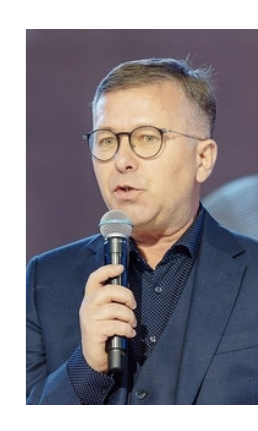
\includegraphics[width=1in,height=1.25in,clip,keepaspectratio]{figs/florin_olariu.png}}]{Florin Olariu}
(Member, IEEE) is currently pursuing the Ph.D. degree with the Faculty of
Computer Science, Alexandru Ioan Cuza University, Ia\c{s}i, Romania. His
research interests include cloud-native architectures, multi-cloud migration
planning, and explainable, constraint-aware decision-support systems for
cloud infrastructure.
\end{IEEEbiography}

\begin{IEEEbiography}[{
\includegraphics[width=1in,height=1.25in,clip,keepaspectratio]{figs/lenuta_alboaie.png}}]{Lenu\c{t}a Alboaie}
(Senior Member, IEEE) is currently an Associate Professor with the Faculty of
Computer Science, Alexandru Ioan Cuza University, Ia\c{s}i, Romania. Her
research interests include distributed systems, cloud computing, and
software architectures.
\end{IEEEbiography}

\begin{IEEEbiography}[{
\includegraphics[width=1in,height=1.25in,clip,keepaspectratio]{figs/cosmin_bonchis.png}}]{Cosmin Bonchi\c{s}}
is an Associate Professor in Computer Science with the Faculty of Computer
Science, West University of Timi\c{s}oara, Timi\c{s}oara, Romania. His
research interests include artificial intelligence and multi-agent systems,
game theory and mechanism design, information theory, optimization, computer
vision, and quantum computing. His current research focuses on algorithmic
and game-theoretic approaches to multi-agent systems, mechanism design with
predictions, and computational methods for intelligent systems.
\end{IEEEbiography}

\end{document}
